% Predicción conforme: guía teórica del repositorio. Las aplicaciones están en ../aplicaciones.
% Compila con pdfLaTeX (por defecto en Overleaf) o XeLaTeX.
\documentclass[11pt]{article}
\usepackage{iftex}
\ifPDFTeX
  \usepackage[utf8]{inputenc}
  \usepackage[T1]{fontenc}
  \IfFileExists{lmodern.sty}{\usepackage{lmodern}}{}
  \IfFileExists{spanish.ldf}%
    {\usepackage[spanish,es-noshorthands,es-nodecimaldot,es-noquoting,es-tabla]{babel}}%
    {\usepackage{babel}\babelprovide[main,import]{spanish}}
\else
  \usepackage{fontspec}
  \usepackage{polyglossia}
  \setdefaultlanguage{spanish}
\fi
\usepackage[margin=2.4cm]{geometry}
\usepackage{amsmath,amssymb,amsthm,mathtools,booktabs,array,enumitem}
\usepackage{graphicx}
\IfFileExists{lmodern.sty}{\usepackage{microtype}}{}
\usepackage[hidelinks]{hyperref}
\usepackage{needspace}
\setlist{itemsep=2pt,topsep=4pt}
\setlength{\parindent}{0pt}
\setlength{\parskip}{5pt}
\setlength{\emergencystretch}{3em}
\theoremstyle{plain}
\newtheorem{teorema}{Teorema}[section]
\newtheorem{lema}[teorema]{Lema}
\newtheorem{proposicion}[teorema]{Proposición}
\newtheorem{corolario}[teorema]{Corolario}
\theoremstyle{definition}
\newtheorem{definicion}[teorema]{Definición}
\newtheorem{ejemplo}[teorema]{Ejemplo}
\theoremstyle{remark}
\newtheorem*{observacion}{Observación}
\renewcommand{\qedsymbol}{$\blacksquare$}
\newcommand{\Prob}{\mathbb P}
\newcommand{\E}{\mathbb E}
\newcommand{\Var}{\operatorname{Var}}
\newcommand{\ind}{\mathbf 1}
\newcommand{\qhat}{\widehat q}
\newcommand{\fhat}{\widehat f_T}
\newcommand{\phat}{\widehat p}
\newcommand{\logit}{\operatorname{logit}}
\newcommand{\eqd}{\overset{d}{=}}
\newcommand{\dest}[1]{\par\needspace{4\baselineskip}\textbf{#1}\quad}
\newcommand{\lamina}[1]{}% marcas de la presentación original; no se imprimen
\title{Predicción conforme\\\large Guía teórica}
\author{José Diego Martínez Hernández}
\date{Octubre de 2026}
\begin{document}
\maketitle
\begin{abstract}
La predicción conforme convierte cualquier modelo en un conjunto predictivo con cobertura marginal
en muestra finita, bajo un solo supuesto: intercambiabilidad de los puntajes. Esta guía sigue la
estructura del tutorial de Angelopoulos y Bates:
primero el objetivo y qué conjuntos queremos, luego un algoritmo concreto con un clasificador de
dígitos, después la receta general con ejemplos de puntajes de no conformidad, el ordenamiento de los
puntajes y la intercambiabilidad como respuesta a por qué todos los huecos son igual de probables. Sólo
entonces, con el supuesto y los puntajes ya presentados, el ejemplo de 19 puntajes y el teorema de
cobertura con su demostración completa. Siguen la diferencia entre cobertura marginal y condicional, la variación entre
calibraciones, el crédito con la cobertura por clase, las elecciones de 2012 como caso principal (con
un umbral por tipo de sección) y los p-valores conformes. El conteo de 2018 queda como complemento. Todas las demostraciones están explícitas. Los
programas de cada ejemplo están en la carpeta \texttt{aplicaciones} del repositorio.
\end{abstract}
\setcounter{tocdepth}{1}
\tableofcontents
\newpage

% =====================================================================
\section{La pregunta y el objetivo}\label{sec:objetivo}\lamina{2--6}
\subsection{Por qué un conjunto}
Un predictor puntual $\widehat f(x)$ responde ``¿qué valor espero?''. Pero en las decisiones importa
también qué otras respuestas son plausibles. Ante un dígito borroso, ``es un 1'' es menos útil que
``es un 1, un 4 o un 5, y la respuesta correcta está en esa lista el 90\% de las veces''. Un conjunto
predictivo $C(x)$ responde ``¿qué respuestas son compatibles con lo aprendido, al nivel de cobertura
elegido?''. Para una respuesta real, $C(x)$ suele ser un intervalo; para una etiqueta, un subconjunto
de etiquetas. La predicción conforme toma la incertidumbre \emph{heurística} de cualquier modelo
(probabilidades, residuos, cuantiles) y la convierte en un conjunto con una garantía precisa
(Angelopoulos y Bates, 2023).

\dest{Confianza y predicción.} Un intervalo de confianza se refiere a un parámetro, como
$\E(Y\mid X=x)$, y se angosta cuando crece la muestra. Un intervalo de predicción se refiere a una
observación nueva: aunque el modelo se conociera sin error, la variabilidad propia de $Y$ no
desaparece. La predicción conforme construye conjuntos de predicción.

\subsection{El objetivo, leído con cuidado}
\dest{Notación.} Los datos son $Z_i=(X_i,Y_i)$. Hay tres bloques: un \emph{entrenamiento} $T$ que
ajusta el modelo; una \emph{calibración} $D_{\rm cal}=\{Z_1,\dots,Z_n\}$ que el modelo no vio y que
fija un umbral; y un \emph{caso nuevo} $Z_{n+1}$ del que sólo se observa $X_{n+1}$. Cualquier
aleatoriedad del ajuste (semillas, validación cruzada) se considera parte de $T$.

El objetivo es que, para un nivel $0<\alpha<1$ elegido de antemano,
\[
 \Prob\{Y_{n+1}\in C(X_{n+1})\}\ge 1-\alpha .
\]
\begin{itemize}
\item $\alpha$ es la tasa de error tolerada: $\alpha=0.10$ pide 90\%.
\item La probabilidad es sobre \emph{todo lo aleatorio}: la calibración y el caso nuevo (y, si no se
condiciona, el entrenamiento). Es una propiedad del procedimiento repetido; no asigna probabilidad
$1-\alpha$ a cada conjunto ya observado ni a cada individuo concreto.
\item Con ``$\ge$'' se habla de cobertura \emph{conservadora}; con ``$=$'', de cobertura
\emph{exacta}.
\item Como promedia sobre todos los casos, se llama cobertura \emph{marginal}. La diferencia con una
cobertura condicional a cada $x$ se discute en la sección~\ref{sec:condicional}.
\end{itemize}

\subsection{Qué conjuntos queremos}
La cobertura sola no basta.
\begin{proposicion}[un conjunto exacto e inútil]
Sea $\mathcal Y$ el espacio de respuestas y $B$ una Bernoulli$(1-\alpha)$ independiente de todo. El
conjunto $C(x)=\mathcal Y$ si $B=1$ y $C(x)=\varnothing$ si $B=0$ tiene cobertura exactamente
$1-\alpha$ para cualquier distribución.
\end{proposicion}
\begin{proof}
$Y_{n+1}\in C(X_{n+1})$ si y sólo si $B=1$, que tiene probabilidad $1-\alpha$.
\end{proof}
Este conjunto no usa los datos y no dice nada. Por eso se piden tres cosas (Angelopoulos y Bates,
2023):
\begin{enumerate}
\item \textbf{Cobertura} al menos $1-\alpha$ y cercana a la exacta.
\item \textbf{Tamaño pequeño}, para que quien decide vea una lista corta de respuestas plausibles.
\item \textbf{Adaptatividad}: conjuntos pequeños para casos fáciles y grandes para casos difíciles,
de modo que el tamaño informe sobre la dificultad.
\end{enumerate}
La calibración se encarga de (1) para cualquier modelo (sección~\ref{sec:teorema}). El modelo y el
puntaje deciden qué tan bien se cumplen (2) y (3) (sección~\ref{sec:puntajes}).

\section{El punto de comparación clásico}
\subsection{Regresión lineal normal}
Sea $\mathbf X$ la matriz de diseño de entrenamiento, de $m\times d$ y rango completo $d<m$, y
supóngase
\[
 Y_i=x_i^\top\beta+\varepsilon_i,\qquad \varepsilon_i\overset{\rm iid}{\sim}N(0,\sigma^2).
\]
\begin{proposicion}
Para una observación nueva $Y=x^\top\beta+\varepsilon$, con $\varepsilon\sim N(0,\sigma^2)$
independiente del entrenamiento, el intervalo
\[
 x^\top\widehat\beta\ \pm\ t_{m-d,1-\alpha/2}\,\widehat\sigma\sqrt{1+x^\top(\mathbf X^\top\mathbf X)^{-1}x}
\]
tiene cobertura exactamente $1-\alpha$, condicionada al diseño y a $x$.
\end{proposicion}
\begin{proof}
Con $\widehat\beta=(\mathbf X^\top\mathbf X)^{-1}\mathbf X^\top\mathbf Y$ se tiene
$\widehat\beta\sim N\bigl(\beta,\sigma^2(\mathbf X^\top\mathbf X)^{-1}\bigr)$. El error de predicción
$e=Y-x^\top\widehat\beta=\varepsilon-x^\top(\widehat\beta-\beta)$ es suma de dos normales
independientes centradas, así que
\[
 e\sim N\bigl(0,\ \sigma^2[1+x^\top(\mathbf X^\top\mathbf X)^{-1}x]\bigr).
\]
El estimador $\widehat\sigma^2=\|\mathbf Y-\mathbf X\widehat\beta\|^2/(m-d)$ cumple
$(m-d)\widehat\sigma^2/\sigma^2\sim\chi^2_{m-d}$ y es independiente de $\widehat\beta$ (teorema de
Cochran: los residuos y los ajustados viven en subespacios ortogonales) y de $\varepsilon$. Por tanto
\[
 \frac{e}{\widehat\sigma\sqrt{1+x^\top(\mathbf X^\top\mathbf X)^{-1}x}}
 =\frac{e/\bigl(\sigma\sqrt{1+x^\top(\mathbf X^\top\mathbf X)^{-1}x}\bigr)}{\sqrt{\widehat\sigma^2/\sigma^2}}
 \sim t_{m-d},
\]
cociente de una normal estándar entre la raíz de una $\chi^2_{m-d}/(m-d)$ independiente. La
probabilidad de que $|t_{m-d}|\le t_{m-d,1-\alpha/2}$ es $1-\alpha$.
\end{proof}
El ``1'' dentro de la raíz es el ruido de la observación nueva; sin él se obtiene el intervalo de
confianza para la media. La exactitud descansa en normalidad, linealidad y homocedasticidad.

\dest{La pregunta de la charla.} ¿Cómo construir un conjunto cuando el predictor es un boosting,
una red o una regresión mal especificada? (Para respuestas binarias, la referencia clásica correspondiente se
presenta junto con el crédito, en la sección~\ref{sec:credito}.) Conformal cambia el fundamento de la garantía: ya no la
saca del modelo, sino de los rangos de puntajes intercambiables. A cambio, la garantía es
marginal, no para cada $x$.

% =====================================================================
\section{Un primer algoritmo: clasificar dígitos}\label{sec:primer}\lamina{7--9}
Antes de la teoría, un algoritmo concreto que se entiende solo.

\dest{Datos.} 1,797 imágenes de dígitos escritos a mano, de $8\times8$ píxeles con intensidades de 0
a 16 (conjunto de dígitos de UCI incluido en \texttt{scikit-learn}). A cada imagen se le asigna al
azar un nivel de ruido gaussiano: ninguno, medio (desviación 4) o alto (desviación 8), recortando a
$[0,16]$. El mismo mecanismo se aplica a entrenamiento, calibración y prueba, así que los datos
siguen siendo intercambiables. Modelo: regresión logística multinomial con penalización, que da
probabilidades $\phat_0(x),\dots,\phat_9(x)$. Particiones al azar de 600 imágenes de entrenamiento,
500 de calibración y 697 de prueba; $\alpha=0.10$.

\dest{El algoritmo.}
\begin{enumerate}
\item Para cada imagen de calibración, anotar la probabilidad que el modelo le dio a la clase
\emph{correcta}: $\phat_{Y_i}(X_i)$, $i=1,\dots,n$.
\item Tomar como umbral $\widehat t$ el valor que deja por debajo a cerca del 10\% de esas
probabilidades. Con la corrección de muestra finita, $\widehat t$ es la $m$-ésima menor de ellas, con
$m=\lfloor\alpha(n+1)\rfloor$; para $n=500$, $m=50$.
\item Para una imagen nueva, $C(x)=\{y:\ \phat_y(x)\ge\widehat t\}$.
\end{enumerate}
\begin{center}
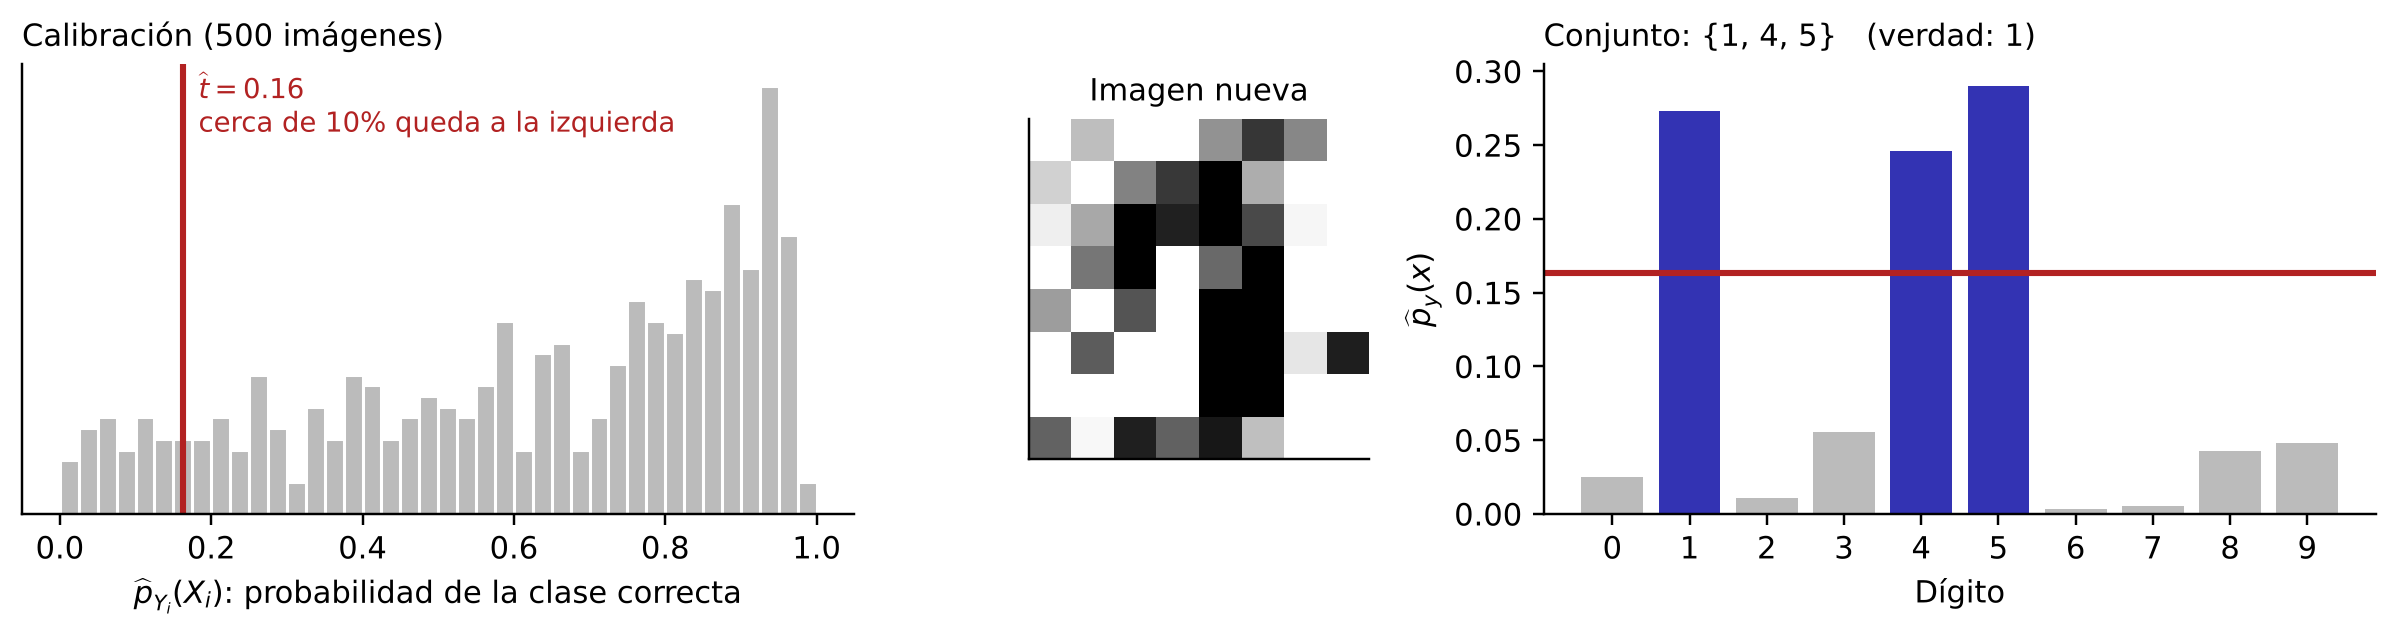
\includegraphics[width=\textwidth]{figuras/imagenes_algoritmo.png}
\end{center}
En la partición mostrada, $\widehat t=0.16$: 9.8\% de las probabilidades de calibración quedaron por
debajo. La imagen nueva recibe las tres etiquetas cuya probabilidad supera la línea: $\{1,4,5\}$.

\dest{El resultado.} En las 697 imágenes de prueba, promediando 100 particiones, el conjunto contiene
la etiqueta correcta 89.9\% de las veces, aunque el modelo sólo acierta con su etiqueta más probable
81\% de las veces. ¿Por qué justo 90\%, sin saber nada del modelo ni de las imágenes? Responder eso
es el objetivo de las secciones~\ref{sec:orden} a \ref{sec:teorema}.

\dest{La intuición.} Si el modelo casi siempre le da probabilidad alta a la clase correcta, el umbral
es alto y los conjuntos son chicos. Si a menudo se equivoca, el umbral baja y los conjuntos crecen.
El conjunto incluye la etiqueta correcta exactamente cuando su probabilidad no cae en el 10\% más bajo,
y si la imagen nueva ``se parece'' a las de calibración, eso pasa 90\% de las veces.

\begin{proposicion}[es split conformal con el puntaje $1-\phat_y$]\label{prop:primer}
Con $s_T(x,y)=1-\phat_y(x)$, $k=\lceil(n+1)(1-\alpha)\rceil\le n$ y $\qhat=S_{(k)}$, se tiene
$\widehat t=1-\qhat$ y $C(x)=\{y: s_T(x,y)\le\qhat\}$.
\end{proposicion}
\begin{proof}
La función $u\mapsto1-u$ invierte el orden: el $k$-ésimo menor de los $S_i=1-\phat_{Y_i}(X_i)$ es uno
menos el $k$-ésimo \emph{mayor} de las probabilidades, que es la $(n+1-k)$-ésima menor. Como
$n+1-k=n+1-\lceil(n+1)(1-\alpha)\rceil=\lfloor\alpha(n+1)\rfloor=m$, resulta $\qhat=1-\widehat t$. Y
$\phat_y(x)\ge\widehat t\iff1-\phat_y(x)\le1-\widehat t=\qhat$.
\end{proof}
Así el primer algoritmo es un caso de la receta general de la sección~\ref{sec:puntajes}, y la garantía
saldrá del Teorema~\ref{teo:split}.

\section{Puntajes de no conformidad}\label{sec:puntajes}\lamina{10--11}
\subsection{La receta general}
El algoritmo de los dígitos es un caso de un procedimiento que sirve para cualquier problema
(Angelopoulos y Bates, 2023):
\begin{enumerate}\setcounter{enumi}{-1}
\item Identificar una noción \emph{heurística} de incertidumbre del modelo: probabilidades, residuos,
cuantiles estimados.
\item Convertirla en un puntaje de no conformidad $s_T(x,y)$.
\item Calcular $\qhat$, el cuantil corregido de los puntajes de calibración (sección~\ref{sec:orden}).
\item Formar el conjunto $C(x)=\{y:\ s_T(x,y)\le\qhat\}$.
\end{enumerate}
En los dígitos, el paso 0 son las probabilidades del modelo y el paso 1 es $s_T=1-\phat_y$
(Proposición~\ref{prop:primer}).

\subsection{La idea}
Un \emph{puntaje de no conformidad} es una función $s_T:\mathcal X\times\mathcal Y\to\mathbb
R\cup\{+\infty\}$, fijada con el entrenamiento, que mide qué tan rara es la respuesta $y$ para el caso
$x$. Valores grandes significan poca compatibilidad. Dado el umbral $\qhat$, el conjunto es siempre
\[
 C(x)=\{y\in\mathcal Y:\ s_T(x,y)\le\qhat\}.
\]
Dos hechos organizan todo lo que sigue.

\begin{proposicion}[la garantía no depende del puntaje]
Para cualquier puntaje fijado con $T$, si los datos son intercambiables dado $T$, el
Teorema~\ref{teo:split} se aplica.
\end{proposicion}
\begin{proof}
El teorema sólo usa que los $S_i=s_T(X_i,Y_i)$ sean intercambiables, y eso lo da el
Lema~\ref{lem:herencia} para cualquier $s_T$ medible fijada con $T$.
\end{proof}

\begin{proposicion}[invariancia ante transformaciones crecientes]\label{prop:monotona}
Si $h$ es estrictamente creciente, usar $h\circ s_T$ en lugar de $s_T$ produce exactamente el mismo
conjunto $C(x)$.
\end{proposicion}
\begin{proof}
Una función estrictamente creciente preserva el orden: el $k$-ésimo menor de los $h(S_i)$ es
$h(S_{(k)})$, así que el nuevo umbral es $h(\qhat)$ (con $h(+\infty)=+\infty$). Y
$h(s_T(x,y))\le h(\qhat)\iff s_T(x,y)\le\qhat$.
\end{proof}
Por eso $1-\phat_y$, $-\phat_y$ y $-\log\phat_y$ dan el mismo conjunto en clasificación. Lo que sí
cambia el conjunto es cambiar \emph{qué se ordena}: residuos absolutos contra residuos escalados,
probabilidad de la etiqueta contra masa acumulada. El puntaje decide la forma y el tamaño de $C(x)$,
es decir, su \emph{utilidad}.

\dest{Receta para invertir un puntaje.} Para saber qué forma tiene $C(x)$ se resuelve la
desigualdad $s_T(x,y)\le\qhat$ en $y$. Los ejemplos siguientes lo hacen explícitamente.

\subsection{Regresión}
\begin{ejemplo}[residuo absoluto]
$s_T(x,y)=|y-\fhat(x)|$. Entonces $|y-\fhat(x)|\le\qhat\iff\fhat(x)-\qhat\le y\le\fhat(x)+\qhat$, y
\[
 C(x)=[\fhat(x)-\qhat,\ \fhat(x)+\qhat].
\]
El ancho $2\qhat$ es el mismo para todo $x$. Si el modelo está mal especificado, $\qhat$ crece y la
banda se ensancha en todas partes, pero la cobertura marginal se conserva.
\end{ejemplo}

\begin{ejemplo}[residuo con signo: intervalos de un lado]
$s_T(x,y)=y-\fhat(x)$ da $C(x)=(-\infty,\fhat(x)+\qhat]$: una cota superior con garantía, útil cuando
sólo importa no subestimar (inventarios, demanda). Con $s_T=\fhat(x)-y$ se obtiene la cota inferior.
\end{ejemplo}

\begin{ejemplo}[residuo escalado]
Con un modelo de escala $\widehat\sigma_T(x)>0$ ajustado en entrenamiento (por ejemplo, una
regresión de $|y-\fhat(x)|$ sobre $x$),
\[
 s_T(x,y)=\frac{|y-\fhat(x)|}{\widehat\sigma_T(x)}\quad\Longrightarrow\quad
 C(x)=[\fhat(x)-\qhat\,\widehat\sigma_T(x),\ \fhat(x)+\qhat\,\widehat\sigma_T(x)].
\]
El ancho es $2\qhat\,\widehat\sigma_T(x)$: mayor donde el modelo espera equivocarse más. Así se
acerca a la cobertura por regiones sin garantizarla.
\end{ejemplo}

\begin{ejemplo}[regresión cuantílica conformalizada, CQR]
Se ajustan en $T$ dos cuantiles condicionales, $\widehat\ell_T(x)\approx q_{\alpha/2}(x)$ y
$\widehat u_T(x)\approx q_{1-\alpha/2}(x)$, y se usa
\[
 s_T(x,y)=\max\{\widehat\ell_T(x)-y,\ y-\widehat u_T(x)\}.
\]
Como el máximo de dos números es $\le\qhat$ si y sólo si ambos lo son,
\[
 s_T(x,y)\le\qhat\iff y\ge\widehat\ell_T(x)-\qhat\ \text{ y }\ y\le\widehat u_T(x)+\qhat
 \iff y\in[\widehat\ell_T(x)-\qhat,\ \widehat u_T(x)+\qhat].
\]
El puntaje es positivo cuando $y$ cae fuera de la banda estimada y negativo cuando cae dentro. Por
eso $\qhat$ puede ser negativo: si la banda estimada era demasiado ancha, la calibración la encoge.
Si los extremos se cruzan el conjunto es vacío; no deben intercambiarse.
\end{ejemplo}

\begin{ejemplo}[proporciones: el voto de una casilla]
Si $y\in(0,1)$ es una proporción, el residuo absoluto puede producir intervalos fuera de $[0,1]$. Con
$\logit(u)=\log\{u/(1-u)\}$ y $\fhat(x)\in(0,1)$,
\[
 s_T(x,y)=|\logit y-\logit\fhat(x)|\quad\Longrightarrow\quad
 C(x)=\bigl[\logit^{-1}(\logit\fhat(x)-\qhat),\ \logit^{-1}(\logit\fhat(x)+\qhat)\bigr],
\]
porque $\logit$ es creciente y biyectiva de $(0,1)$ en $\mathbb R$. El intervalo queda dentro de
$(0,1)$ y es asimétrico: más angosto cerca de cero o de uno. Si $y$ puede valer exactamente 0 o 1, se
aplica antes un pequeño corrimiento fijo.
\end{ejemplo}

\begin{ejemplo}[densidad predictiva]
Si el modelo da una densidad condicional $\widehat p_T(y\mid x)$, el puntaje
$s_T(x,y)=-\widehat p_T(y\mid x)$ produce
\[
 C(x)=\{y:\ \widehat p_T(y\mid x)\ge-\qhat\},
\]
un conjunto de nivel de la densidad (la región de mayor densidad). Con una densidad bimodal puede ser
la unión de dos intervalos: el conjunto no tiene por qué ser un intervalo. Una predictiva bayesiana
sirve igual, y así una predictiva posterior recibe una garantía frecuentista (Fong y Holmes, 2021).
\end{ejemplo}

\begin{ejemplo}[función de distribución predictiva]
Si el modelo da una distribución condicional $\widehat F_T(y\mid x)$ continua y creciente en $y$,
$s_T(x,y)=|\widehat F_T(y\mid x)-1/2|$ da
\[
 C(x)=\bigl[\widehat F_T^{-1}(\tfrac12-\qhat\mid x),\ \widehat F_T^{-1}(\tfrac12+\qhat\mid x)\bigr],
\]
un intervalo entre dos cuantiles predictivos cuyo nivel corrige la calibración (Chernozhukov,
Wüthrich y Zhu, 2021).
\end{ejemplo}

\subsection{Clasificación}
Con $K$ etiquetas y probabilidades estimadas $\phat_1(x),\dots,\phat_K(x)$ que suman uno:

\begin{ejemplo}[probabilidad de la etiqueta, LAC]
$s_T(x,y)=1-\phat_y(x)$. Entonces
\[
 C(x)=\{y:\ 1-\phat_y(x)\le\qhat\}=\{y:\ \phat_y(x)\ge1-\qhat\}:
\]
entra toda etiqueta cuya probabilidad supera el umbral $1-\qhat$. Entre todos los conjuntos con
cobertura marginal $1-\alpha$, éste minimiza el tamaño esperado cuando las probabilidades son las
verdaderas (Sadinle, Lei y Wasserman, 2019). Puede dar conjuntos vacíos: si ninguna etiqueta supera
$1-\qhat$. Es el puntaje de las imágenes y del crédito.
\end{ejemplo}

\begin{ejemplo}[masa acumulada, APS]
Se ordenan las etiquetas de mayor a menor probabilidad y
\[
 s_T(x,y)=\sum_{j:\ \phat_j(x)\ge\phat_y(x)}\phat_j(x),
\]
la masa acumulada hasta llegar a $y$ incluyéndola. Como el puntaje crece al bajar en el orden, el
conjunto $\{y: s_T(x,y)\le\qhat\}$ está formado por las etiquetas más probables mientras la masa
acumulada no rebase $\qhat$. Un caso ambiguo, con la masa repartida, recibe más etiquetas que con
LAC; uno claro, menos. Romano, Sesia y Candès (2020) usan una versión con un desempate aleatorio
que acerca la cobertura al nivel exacto.
\end{ejemplo}

\begin{ejemplo}[vecino más cercano]
Sin probabilidades: con distancias en $\mathcal X$,
\[
 s_T(x,y)=\frac{\text{distancia de $x$ al vecino más cercano en $T$ con etiqueta $y$}}
 {\text{distancia de $x$ al vecino más cercano en $T$ con etiqueta distinta de $y$}}.
\]
Una etiqueta es rara si $x$ está lejos de los ejemplos de esa etiqueta y cerca de los de otras. Es el
ejemplo clásico de Shafer y Vovk (2008).
\end{ejemplo}

\dest{Qué es ``no sé''.} Con dos etiquetas, $C(x)=\{0,1\}$ significa que el modelo no distingue lo
suficiente para comprometerse. Con diez, $\{2,3,6,8\}$ dice ``es alguno de estos cuatro''. El tamaño
del conjunto es una medida honesta de la incertidumbre del modelo en ese caso.

% =====================================================================
\section{Ordenar los puntajes de calibración}\label{sec:orden}\lamina{12--14}
\subsection{Estadísticos de orden y rangos}
Dados los puntajes de calibración $S_1,\dots,S_n$, sus \emph{estadísticos de orden} son los mismos
valores ordenados de menor a mayor:
\[
 S_{(1)}\le S_{(2)}\le\cdots\le S_{(n)}.
\]
$S_{(1)}$ es el mínimo, $S_{(n)}$ el máximo, y $S_{(k)}$ es el $k$-ésimo valor más chico. Si hay
valores repetidos, aparecen repetidos en la lista.

El \emph{rango} del puntaje nuevo entre los $n+1$ puntajes es
\[
 R_{n+1}=1+\#\{i\le n:\ S_i<S_{n+1}\}.
\]
Cuenta cuántos puntajes de calibración quedan estrictamente por debajo del nuevo y le suma uno. Si
$S_{n+1}$ es el más chico de todos, $R_{n+1}=1$; si es el más grande, $R_{n+1}=n+1$.

\dest{Los huecos.} Sin empates, los $n$ puntajes de calibración parten la recta en $n+1$ huecos:
\[
 (-\infty,S_{(1)}),\ (S_{(1)},S_{(2)}),\ \dots,\ (S_{(n-1)},S_{(n)}),\ (S_{(n)},\infty).
\]
El puntaje nuevo cae en exactamente uno de ellos, y el número de ese hueco (contando desde la
izquierda) es su rango: si cae en el hueco $r$, hay exactamente $r-1$ puntajes de calibración por
debajo. Con 19 puntajes hay 20 huecos.

\subsection{El lema de conteo}
Todo el método descansa en traducir ``quedar por debajo del $k$-ésimo'' a ``tener rango a lo más $k$''.
\begin{lema}[conteo]\label{lem:conteo}
Sea $1\le k\le n$. Para todo número real $s$,
\[
 s\le S_{(k)}\quad\iff\quad\#\{i\le n:\ S_i<s\}\le k-1 .
\]
\end{lema}
\begin{proof}
($\Rightarrow$) Si $s\le S_{(k)}$, todo $S_i<s$ cumple $S_i<S_{(k)}$. Los valores
$S_{(k)},S_{(k+1)},\dots,S_{(n)}$ son $n-k+1$ puntajes mayores o iguales que $S_{(k)}$, así que a lo
más $n-(n-k+1)=k-1$ puntajes son estrictamente menores que $S_{(k)}$, y con mayor razón a lo más
$k-1$ son menores que $s$.

($\Leftarrow$) Por contrapositiva: si $s>S_{(k)}$, entonces $S_{(1)}\le\cdots\le S_{(k)}<s$, y hay al
menos $k$ puntajes menores que $s$.
\end{proof}
Aplicado a $s=S_{n+1}$ y usando la definición del rango:
\begin{corolario}\label{cor:cubrir}
Si $1\le k\le n$, $\ \{S_{n+1}\le S_{(k)}\}=\{R_{n+1}\le k\}$, con o sin empates.
\end{corolario}
Es decir: \emph{cubrir es caer en uno de los primeros $k$ huecos}.

\subsection{Por qué el cuantil lleva $n+1$}
La forma natural de escribir el umbral es como un cuantil de la distribución empírica de los
puntajes, \emph{agregando un punto en $+\infty$ que representa al caso nuevo}.
\begin{proposicion}\label{prop:cuantil}
Sea $\widehat F$ la distribución que pone masa $1/(n+1)$ en cada $S_i$ y masa $1/(n+1)$ en $+\infty$.
Su cuantil $1-\alpha$, $\inf\{s:\widehat F(s)\ge1-\alpha\}$, es
\[
 \qhat=\begin{cases}S_{(k)},&k\le n,\\+\infty,&k=n+1,\end{cases}\qquad k=\lceil(n+1)(1-\alpha)\rceil.
\]
\end{proposicion}
\begin{proof}
Para $s$ finito, $\widehat F(s)=\#\{i:S_i\le s\}/(n+1)$. Así, $\widehat F(s)\ge1-\alpha$ equivale a
$\#\{i:S_i\le s\}\ge(n+1)(1-\alpha)$, y como el conteo es entero, a $\#\{i:S_i\le s\}\ge k$. El menor
$s$ que deja al menos $k$ puntajes en $(-\infty,s]$ es $S_{(k)}$ si $k\le n$. Si $k=n+1$, ningún $s$
finito acumula $n+1$ puntajes de calibración, y el ínfimo se alcanza en $+\infty$.
\end{proof}
El punto en $+\infty$ es la manera de ``hacer lugar'' al caso nuevo, cuyo puntaje desconocemos: se
supone lo peor. Con el cuantil ingenuo de los $n$ puntajes, $k_{\rm ing}=\lceil n(1-\alpha)\rceil$,
se ignora ese lugar y la cobertura puede quedar por debajo de $1-\alpha$ (sección~\ref{sec:finita}).

\dest{Por qué no se interpola.} Los paquetes estadísticos suelen interpolar entre estadísticos de
orden. Interpolar puede dar un umbral menor que $S_{(k)}$ y romper la cota inferior. La garantía es
para el estadístico de orden exacto.

\dest{Empates.} Si hay valores repetidos, el conjunto usa ``$\le$'': se incluye toda respuesta cuyo
puntaje empate con $\qhat$. Esa convención es conservadora: sólo puede aumentar la cobertura. La
sección~\ref{sec:teorema} lo prueba.

% =====================================================================
\dest{La pregunta que queda.} Ya sabemos \emph{qué} huecos cubren: los primeros $k$. Falta saber con
qué probabilidad cae el caso nuevo en cada uno. Eso no lo dice el ordenamiento; lo dice el supuesto
de la sección siguiente.

% =====================================================================
\section{Intercambiabilidad: por qué los huecos son igual de probables}\label{sec:intercambiabilidad}
La sección anterior terminó con una pregunta: los $n$ puntajes de calibración parten la recta en
$n+1$ huecos y el caso nuevo cae en uno; cubrir es caer en los primeros $k$. ¿Con qué probabilidad cae
en cada hueco? La respuesta es $1/(n+1)$ para todos, y el supuesto que la produce es la
intercambiabilidad. La probabilidad es sobre la calibración y el caso nuevo juntos; no es la
probabilidad de cada hueco para unos puntajes de calibración ya observados.


\begin{definicion}
Un vector aleatorio $(Z_1,\dots,Z_{N})$ es \emph{intercambiable} si para toda permutación $\pi$ de
$\{1,\dots,N\}$
\[
 (Z_1,\dots,Z_N)\ \eqd\ (Z_{\pi(1)},\dots,Z_{\pi(N)}).
\]
\end{definicion}
Equivalentemente, la ley conjunta es simétrica: ninguna posición es especial. En particular todas las
$Z_i$ tienen la misma marginal y todos los pares $(Z_i,Z_j)$, $i\ne j$, la misma ley conjunta.

\begin{proposicion}[i.i.d.\ implica intercambiable]
Si $Z_1,\dots,Z_N$ son i.i.d.\ con ley $P$, son intercambiables.
\end{proposicion}
\begin{proof}
La ley conjunta es el producto $P\otimes\cdots\otimes P$. Para conjuntos medibles $A_1,\dots,A_N$,
$\Prob(Z_{\pi(1)}\in A_1,\dots,Z_{\pi(N)}\in A_N)=\prod_i P(A_i)=\Prob(Z_1\in A_1,\dots,Z_N\in A_N)$,
porque el producto no depende del orden. Como los rectángulos generan la $\sigma$-álgebra producto,
las dos leyes coinciden.
\end{proof}

\begin{proposicion}[la urna]\label{prop:urna}
Sea una población finita de $M$ unidades con valores $a_1,\dots,a_M$. Si se extraen $N\le M$
unidades al azar y sin reemplazo, los valores extraídos $(Z_1,\dots,Z_N)$ son intercambiables, pero
no independientes.
\end{proposicion}
\begin{proof}
Cada sucesión ordenada de $N$ unidades distintas $(u_1,\dots,u_N)$ tiene probabilidad
$\frac{1}{M}\cdot\frac1{M-1}\cdots\frac1{M-N+1}=\frac{(M-N)!}{M!}$, la misma para todas. Permutar las
posiciones manda sucesiones de unidades distintas en sucesiones de unidades distintas de manera
biyectiva, de modo que la ley de los índices extraídos es invariante; también lo es la de sus
valores. Para la dependencia: si los valores son distintos, $\Prob(Z_2=a_1\mid Z_1=a_1)=0\ne1/M$.
\end{proof}
Ésta es la situación del conteo rápido \emph{dentro de un estrato}: las casillas se sortean sin
reemplazo. También la de 2012 en la sección~\ref{sec:beta2012}: cada calibración es una muestra
al azar de la población de casillas.

\dest{Lo que rompe la simetría.} Series con tendencia; datos ordenados por hora de llegada;
calibración de una población y prueba de otra. En todos ellos alguna posición es especial. La
intercambiabilidad no se verifica mirando si los datos ``se parecen''; se justifica por el
mecanismo que los produce: un sorteo, una partición al azar.

\begin{lema}[los puntajes heredan la simetría]\label{lem:herencia}
Si $(Z_1,\dots,Z_{n+1})$ es intercambiable condicionado a $T$ y $s_T$ es una función medible fijada
con $T$, entonces $S_i=s_T(Z_i)$, $i=1,\dots,n+1$, es intercambiable condicionado a $T$.
\end{lema}
\begin{proof}
Fijemos $T$ y sea $g(z_1,\dots,z_{n+1})=(s_T(z_1),\dots,s_T(z_{n+1}))$. Para una permutación $\pi$,
sea $\sigma_\pi(z_1,\dots,z_{n+1})=(z_{\pi(1)},\dots,z_{\pi(n+1)})$. Aplicar $s_T$ coordenada a
coordenada y permutar conmutan: $g\circ\sigma_\pi=\sigma_\pi\circ g$. Entonces
\[
 \sigma_\pi(S)=\sigma_\pi(g(Z))=g(\sigma_\pi(Z))\ \eqd\ g(Z)=S,
\]
donde la igualdad en distribución usa que $\sigma_\pi(Z)\eqd Z$ dado $T$ y que $g$ es una función
fija dado $T$.
\end{proof}

\dest{Por qué se separan los datos.} El lema exige que $s_T$ sea \emph{la misma} función en todas
las posiciones y que no dependa de las respuestas de calibración. Si se calibrara con residuos de
entrenamiento, esos puntos ya fueron usados para ajustar y sus residuos tienden a ser más chicos que
el del caso nuevo: la posición del caso nuevo sería especial. Lo mismo ocurre si se eligen el modelo,
los hiperparámetros o el puntaje mirando la calibración.

% =====================================================================
\section{El ejemplo de 19 puntajes, a fondo}\label{sec:ej19}\lamina{15}
\subsection{El cálculo}
Sea $n=19$ y $\alpha=0.10$. Primero el orden:
\[
 k=\lceil(19+1)(1-0.10)\rceil=\lceil18\rceil=18\le19,
\]
así que el umbral es el decimoctavo puntaje más chico. Supongamos que los errores absolutos de
calibración, ya ordenados, son
\[
 0.1,\ 0.2,\ 0.3,\ \dots,\ 1.7,\ 1.8,\ 2.4,
\]
es decir, $S_{(j)}=j/10$ para $j=1,\dots,18$ y $S_{(19)}=2.4$. Entonces $\qhat=S_{(18)}=1.8$. Con el
puntaje $|y-\fhat(x)|$ y una predicción $\fhat(x)=5$:
\[
 C(x)=[5-1.8,\ 5+1.8]=[3.2,\ 6.8].
\]
El puntaje más grande, $2.4$, no influye: el umbral ignora al peor de los 19. Si en lugar de $2.4$
hubiera sido $240$, el intervalo sería el mismo.

\subsection{Dónde puede caer el caso nuevo}
Sea $e=|Y_{n+1}-\fhat(X_{n+1})|$ el error del caso nuevo. La tabla recorre los 20 huecos:
\begin{center}
\renewcommand{\arraystretch}{1.25}
\begin{tabular}{ccccc}
\toprule
Hueco (rango) & Valores de $e$ & Puntajes de calibración menores & ¿$e\le1.8$? & ¿Cubre?\\
\midrule
1 & $e<0.1$ & 0 & sí & sí\\
2 & $0.1<e<0.2$ & 1 & sí & sí\\
$\vdots$ & $\vdots$ & $\vdots$ & $\vdots$ & $\vdots$\\
18 & $1.7<e<1.8$ & 17 & sí & sí\\
19 & $1.8<e<2.4$ & 18 & no & no\\
20 & $e>2.4$ & 19 & no & no\\
\bottomrule
\end{tabular}
\end{center}
Exactamente los primeros 18 huecos cubren, como dice el Corolario~\ref{cor:cubrir}. Bajo
intercambiabilidad, y sin empates, el caso nuevo tiene la misma probabilidad de caer en cualquiera de
los 20 (Lema~\ref{lem:rango}), así que cubre con probabilidad $18/20=0.90$.

\subsection{Lo que el ejemplo no dice}
\dest{El 90\% no es de esta calibración.} La probabilidad $18/20$ promedia sobre \emph{todas} las
calibraciones posibles y sobre el caso nuevo. Una vez que los 19 puntajes son estos, la cobertura del
intervalo $[3.2,6.8]$ es un número fijo: la probabilidad de que un error nuevo sea menor que $1.8$.
Si la distribución verdadera de los errores fuera, por ejemplo, exponencial con media $0.6$, ese
número sería $1-e^{-1.8/0.6}=0.950$; si la media fuera $1$, sería $1-e^{-1.8}=0.835$. Al repetir la
calibración, este número varía alrededor de $0.90$ con ley Beta (sección~\ref{sec:beta}).

\dest{Qué pasa al cambiar $n$ o $\alpha$.}
\begin{itemize}
\item Con $n=18$: $k=\lceil19\times0.9\rceil=\lceil17.1\rceil=18$, el umbral es el máximo
$S_{(18)}$ y la cobertura sin empates es $18/19\approx0.947$. No siempre se puede llegar exactamente a
$0.90$: los niveles alcanzables son múltiplos de $1/(n+1)$.
\item Con $\alpha=0.05$ y $n=19$: $k=\lceil19\rceil=19$, el umbral es el máximo $2.4$ y el intervalo
es $[2.6,7.4]$, con cobertura $19/20=0.95$.
\item Con $\alpha=0.05$ y $n=18$: $k=\lceil18.05\rceil=19>18$, el umbral es $+\infty$ y el conjunto es
toda la recta. Con 18 datos no se puede prometer 95\% de manera informativa.
\end{itemize}

\dest{El cuantil ingenuo.} Con los mismos 19 puntajes, el cuantil 90\% ``de libro'' sin el $n+1$ usa
$\lceil19\times0.9\rceil=\lceil17.1\rceil=18$: coincide por casualidad. Con $n=10$, en cambio, el ingenuo
usa $k=9$ y cubre $9/11\approx0.818$, mientras que el corregido usa $k=10$ y cubre $10/11\approx0.909$.

\dest{Empates en el ejemplo.} Si dos puntajes valieran $1.8$, por ejemplo $S_{(17)}=S_{(18)}=1.8$, el
umbral seguiría siendo $1.8$ y el intervalo el mismo. Un error nuevo exactamente igual a $1.8$ queda
cubierto por la convención ``$\le$''. Con errores continuos esto tiene probabilidad cero; con puntajes
discretos (por ejemplo, árboles con pocas hojas) puede pasar y sólo aumenta la cobertura.

% =====================================================================
\section{El teorema y su demostración}\label{sec:teorema}\lamina{16}
\subsection{El algoritmo completo}
\begin{enumerate}
\item Con el entrenamiento $T$: ajustar el modelo y fijar el puntaje $s_T$.
\item Con la calibración: calcular $S_i=s_T(X_i,Y_i)$, $i=1,\dots,n$, y ordenarlos.
\item Con $k=\lceil(n+1)(1-\alpha)\rceil$: tomar $\qhat=S_{(k)}$ si $k\le n$, y $\qhat=+\infty$ si
$k=n+1$.
\item Para el caso nuevo: $C(X_{n+1})=\{y:\ s_T(X_{n+1},y)\le\qhat\}$.
\end{enumerate}

\subsection{El rango es uniforme}
Para cada posición $j\in\{1,\dots,n+1\}$ definimos su rango entre los $n+1$ puntajes,
\[
 R_j=1+\#\{i\ne j:\ S_i<S_j\},
\]
de modo que $R_{n+1}$ es el rango del caso nuevo de la sección~\ref{sec:orden}.
\begin{lema}[rango uniforme]\label{lem:rango}
Si $(S_1,\dots,S_{n+1})$ es intercambiable dado $T$ y los puntajes, con valores en un conjunto con
orden total (números reales o pares en orden lexicográfico), son distintos casi seguramente, entonces
para cada $j$
\[
 \Prob(R_j=r\mid T)=\frac1{n+1},\qquad r=1,\dots,n+1.
\]
\end{lema}
\begin{proof}
\emph{Paso 1: los rangos son una permutación.} Si los $n+1$ puntajes son distintos, ordenarlos asigna
a cada uno una posición distinta del $1$ al $n+1$, y esa posición es exactamente $R_j$. Así,
$(R_1,\dots,R_{n+1})$ es una permutación de $\{1,\dots,n+1\}$, y para cada $r$
\[
 \sum_{j=1}^{n+1}\ind\{R_j=r\}=1 .
\]

\emph{Paso 2: todas las posiciones tienen la misma ley de rango.} Fijemos $j$ y sea $\pi$ la
transposición que intercambia $j$ y $n+1$. El rango es una función de todo el vector,
$R_j=\rho_j(S_1,\dots,S_{n+1})$, y permutar el vector intercambia los papeles:
$\rho_{n+1}(S_{\pi(1)},\dots,S_{\pi(n+1)})=\rho_j(S_1,\dots,S_{n+1})$. Por intercambiabilidad
$(S_{\pi(1)},\dots,S_{\pi(n+1)})\eqd(S_1,\dots,S_{n+1})$ dado $T$, así que
\[
 \Prob(R_{n+1}=r\mid T)=\Prob\bigl(\rho_{n+1}(S_\pi)=r\mid T\bigr)=\Prob(\rho_j(S)=r\mid T)=\Prob(R_j=r\mid T).
\]

\emph{Paso 3: cada una vale $1/(n+1)$.} Tomando esperanza condicional en el paso 1,
$\sum_{j}\Prob(R_j=r\mid T)=1$. Los $n+1$ sumandos son iguales por el paso 2, así que cada uno vale
$1/(n+1)$.
\end{proof}

\subsection{El teorema}
\begin{teorema}[cobertura de split conformal]\label{teo:split}
Si los puntajes $(S_1,\dots,S_{n+1})$ son intercambiables dado $T$, entonces
\[
 \Prob\{Y_{n+1}\in C(X_{n+1})\mid T\}\ \ge\ \frac{k}{n+1}\ \ge\ 1-\alpha .
\]
Si además son distintos casi seguramente, la primera desigualdad es una igualdad y
\[
 1-\alpha\ \le\ \Prob\{Y_{n+1}\in C(X_{n+1})\mid T\}\ <\ 1-\alpha+\frac1{n+1}.
\]
Las mismas cotas valen sin condicionar a $T$.
\end{teorema}

\begin{proof}[Demostración sin empates]
\emph{Caso $k=n+1$.} Entonces $\qhat=+\infty$, el conjunto es todo el espacio y la cobertura es
$1=k/(n+1)$.

\emph{Caso $k\le n$.} Por definición del conjunto y del umbral,
$\{Y_{n+1}\in C(X_{n+1})\}=\{s_T(X_{n+1},Y_{n+1})\le\qhat\}=\{S_{n+1}\le S_{(k)}\}$, y por el
Corolario~\ref{cor:cubrir} esto es $\{R_{n+1}\le k\}$. Por el Lema~\ref{lem:rango},
\[
 \Prob\{Y_{n+1}\in C(X_{n+1})\mid T\}=\sum_{r=1}^{k}\Prob(R_{n+1}=r\mid T)=\frac{k}{n+1}.
\]

\emph{Las cotas.} Como $k$ es el menor entero mayor o igual que $(n+1)(1-\alpha)$,
\[
 (n+1)(1-\alpha)\ \le\ k\ <\ (n+1)(1-\alpha)+1 .
\]
Dividiendo entre $n+1$: $1-\alpha\le k/(n+1)<1-\alpha+1/(n+1)$.

\emph{Sin condicionar.} Por la ley de la esperanza total,
$\Prob\{Y_{n+1}\in C(X_{n+1})\}=\E\bigl[\Prob\{Y_{n+1}\in C(X_{n+1})\mid T\}\bigr]$, y las cotas, que
no dependen de $T$, pasan al promedio.
\end{proof}

\begin{proof}[Demostración de la cota inferior con empates]
Si $k=n+1$ no hay nada que probar. Sea $k\le n$. Tomemos $U_1,\dots,U_{n+1}$ i.i.d.\ uniformes en
$(0,1)$, independientes de los datos y de $T$, y ordenemos los pares $(S_i,U_i)$
lexicográficamente: primero por puntaje y, si empatan, por $U_i$. Los pares son intercambiables dado
$T$ (el vector de pares es la imagen del vector intercambiable $((Z_i,U_i))_i$) y distintos casi
seguramente, porque dos $U$ coinciden con probabilidad cero. Su rango
\[
 R^*_{n+1}=1+\#\{i\le n:\ (S_i,U_i)<(S_{n+1},U_{n+1})\}
\]
es uniforme por el Lema~\ref{lem:rango}. Si $S_i<S_{n+1}$ entonces $(S_i,U_i)<(S_{n+1},U_{n+1})$, así
que
\[
 R_{n+1}=1+\#\{i\le n:\ S_i<S_{n+1}\}\ \le\ R^*_{n+1}.
\]
Por tanto $\{R^*_{n+1}\le k\}\subseteq\{R_{n+1}\le k\}=\{S_{n+1}\le S_{(k)}\}$, la última igualdad por
el Corolario~\ref{cor:cubrir}, que vale con empates. Así
\[
 \Prob\{Y_{n+1}\in C(X_{n+1})\mid T\}\ \ge\ \Prob(R^*_{n+1}\le k\mid T)=\frac{k}{n+1}\ \ge\ 1-\alpha.
\]
El desempate es sólo un artificio de la prueba: el conjunto que se usa en la práctica no cambia.
\end{proof}

\dest{Por qué con empates no hay cota superior.} La regla ``$\le$'' incluye los empates con el
umbral, lo que sólo puede aumentar la cobertura. En el extremo, si los $n+1$ puntajes son iguales
casi seguramente, el conjunto cubre siempre. Un procedimiento que use explícitamente el desempate al
predecir recupera la igualdad $k/(n+1)$, a costa de aleatorizar la inclusión de etiquetas.

\dest{Lo que la prueba no usó.} Que el modelo sea correcto, normalidad, independencia, ni $n$ grande.
Sólo intercambiabilidad de los puntajes. Y la cota superior dice que la garantía no es holgada: sin
empates el procedimiento cubre entre $1-\alpha$ y $1-\alpha+1/(n+1)$.

\dest{Exactitud.} ``Exacto en muestra finita'' significa que la garantía no depende de un límite.
La igualdad con $1-\alpha$ requiere además que $(n+1)(1-\alpha)$ sea entero; en otro caso la
cobertura sin empates es $k/(n+1)$, ligeramente mayor.

% =====================================================================
\section{Muestra finita}\label{sec:finita}
\subsection{El cuantil ingenuo cubre de menos}
Con el cuantil ingenuo $k_{\rm ing}=\lceil n(1-\alpha)\rceil$, el mismo argumento da cobertura sin
empates $k_{\rm ing}/(n+1)$:
\begin{center}
\begin{tabular}{rcccc}
\toprule
$n$ & $k_{\rm ing}$ & Cobertura ingenua & $k$ & Cobertura corregida\\
\midrule
10&9&$9/11=81.82\%$&10&$10/11=90.91\%$\\
19&18&$18/20=90\%$&18&$18/20=90\%$\\
50&45&$45/51=88.24\%$&46&$46/51=90.20\%$\\
100&90&$90/101=89.11\%$&91&$91/101=90.10\%$\\
\bottomrule
\end{tabular}
\end{center}

\subsection{Tamaño mínimo de calibración}
\begin{proposicion}
El umbral es finito ($k\le n$) si y sólo si $n\ge1/\alpha-1$.
\end{proposicion}
\begin{proof}
Para $n$ entero, $\lceil x\rceil\le n\iff x\le n$. Así $k\le n\iff(n+1)(1-\alpha)\le n\iff
n+1-\alpha(n+1)\le n\iff1\le\alpha(n+1)\iff n\ge1/\alpha-1$.
\end{proof}
Con $\alpha=0.10$ se necesitan al menos 9 datos; con $\alpha=0.05$, 19; con $\alpha=0.01$, 99. La
condición sólo evita el conjunto trivial; no asegura que el conjunto sea útil. Además, sin empates
sólo son alcanzables las coberturas $1/(n+1),2/(n+1),\dots,1$.

\section{Volvamos a los dígitos: tamaño y grupos}\label{sec:imagenes}\lamina{9}
\begin{center}
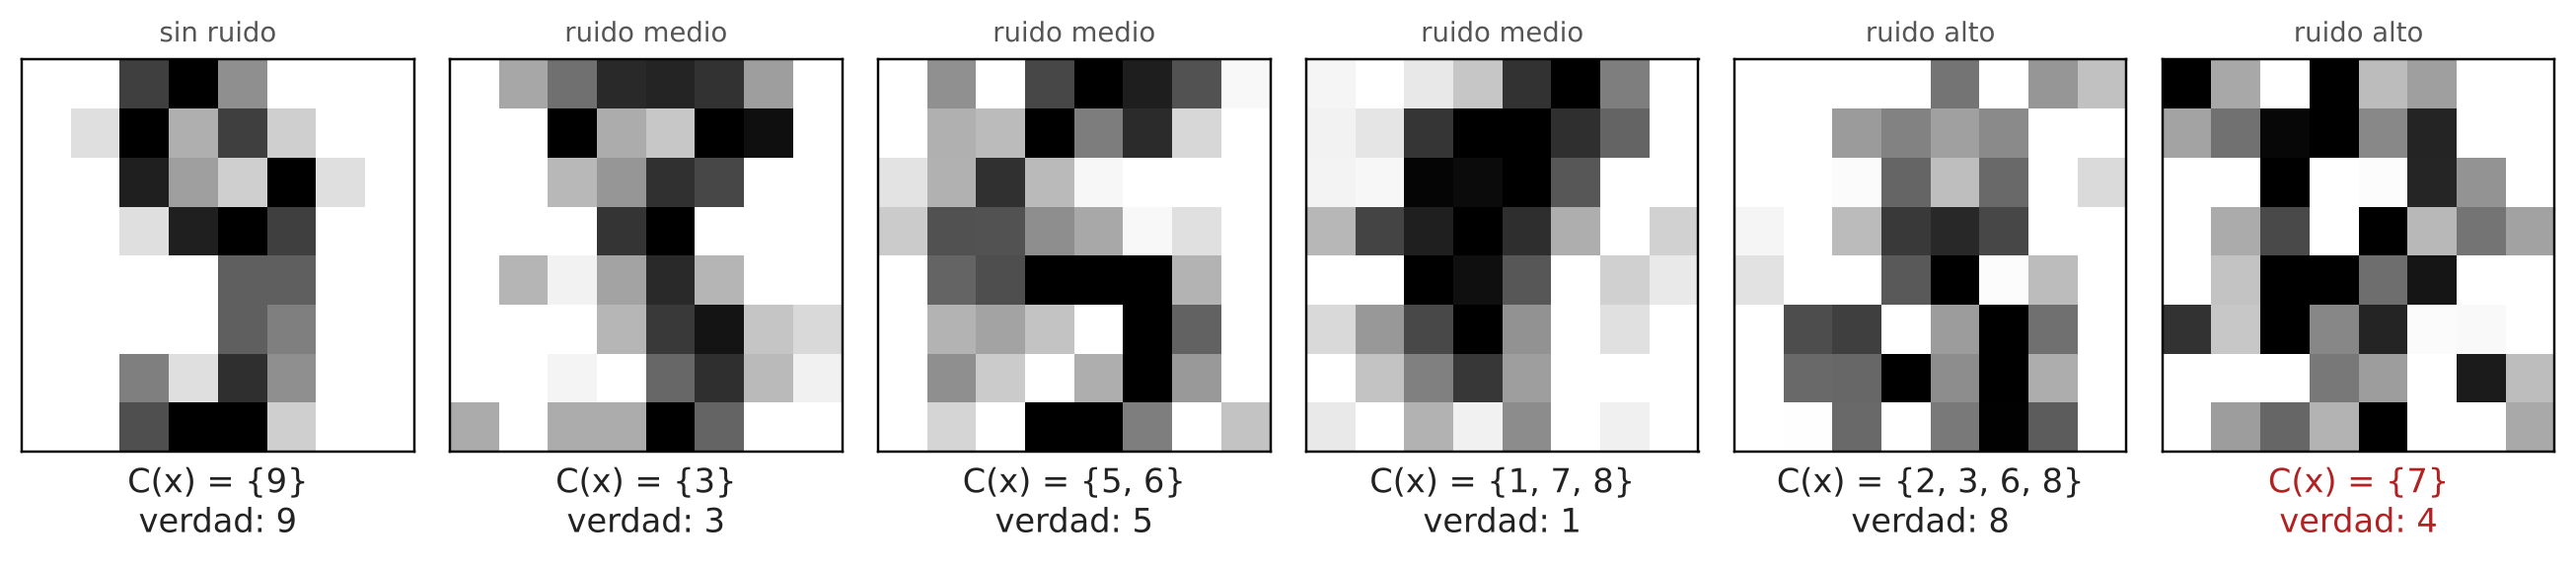
\includegraphics[width=\textwidth]{figuras/imagenes_ejemplos.png}
\end{center}
En la partición mostrada el umbral fue $\qhat=0.84$: entra al conjunto toda etiqueta con
probabilidad estimada de al menos $0.16$. Una imagen clara recibe una sola etiqueta; una borrosa,
varias. El caso en rojo es un fallo: el modelo le dio 0.56 a un 7 y era un 4. Fallar en 10\% de los
casos es parte del contrato.
\begin{center}
\begin{tabular}{lcccc}
\toprule
& Todas & Sin ruido & Ruido medio & Ruido alto\\
\midrule
Cobertura & 89.9\% & 97.1\% & 94.2\% & 78.6\%\\
Tamaño medio del conjunto & 1.40 & 1.23 & 1.36 & 1.60\\
Conjuntos de una etiqueta & 66.0\% & 79.7\% & 68.7\% & 49.8\%\\
Exactitud del modelo & 80.9\% & 92.7\% & 86.4\% & 63.6\%\\
\bottomrule
\end{tabular}
\end{center}
Medias de 100 particiones; el error Monte Carlo de la cobertura global es 0.17 puntos. En promedio
$\qhat=0.82$; los conjuntos vacíos aparecen en 0.08\% de los casos.

\dest{Lectura.} En términos de los tres deseables de la sección~\ref{sec:objetivo}:
\begin{enumerate}
\item \emph{Cobertura}: la global es la prometida, aunque el modelo sólo acierta 81\% de las veces.
El conjunto compensa con tamaño lo que el modelo no sabe.
\item \emph{Tamaño}: 1.4 etiquetas en promedio, de diez posibles.
\item \emph{Adaptatividad}: más ruido, más etiquetas. Pero la cobertura no es 90\% en cada grupo: las
imágenes limpias se cubren de más (97\%) y las más borrosas de menos (79\%). El promedio esconde la
diferencia; es el tema de la sección siguiente.
\end{enumerate}

\section{Cobertura marginal y cobertura condicional}\label{sec:condicional}
\subsection{Las dos garantías}
La garantía del Teorema~\ref{teo:split} es \emph{marginal}:
\[
 \Prob\{Y_{n+1}\in C(X_{n+1})\}\ge1-\alpha ,
\]
un promedio sobre todos los casos. La garantía deseable sería \emph{condicional}:
\[
 \Prob\{Y_{n+1}\in C(X_{n+1})\mid X_{n+1}=x\}\ge1-\alpha\quad\text{para casi todo }x .
\]
La condicional implica la marginal (promediando sobre $x$), pero no al revés. Con dos grupos:
\begin{center}
\begin{tabular}{lccc}
\toprule
& Sin garantía & Marginal & Condicional\\
\midrule
Grupo 1 (80\% de los casos) & 75\% & 100\% & 90\%\\
Grupo 2 (20\% de los casos) & 60\% & 50\% & 90\%\\
Global & 72\% & 90\% & 90\%\\
\bottomrule
\end{tabular}
\end{center}
La columna del centro cumple la garantía marginal porque $0.8\times1+0.2\times0.5=0.90$, aunque un
grupo se cubra a la mitad. El fenómeno aparece en los tres ejemplos: las imágenes más borrosas se
cubren al 79\%, los incumplidores al 56--58\% y las casillas rurales alrededor del 75\%.

\dest{Lo que no se puede pedir.} Para una respuesta real, si un procedimiento garantiza cobertura
condicional para \emph{toda} distribución, entonces para casi todo punto $x$ (respecto de la
distribución de $X$) que no sea un átomo, la longitud esperada del conjunto es infinita (Vovk, 2012;
Lei y Wasserman, 2014; Foygel Barber et al., 2021). La intuición: con $X$ continua no hay datos en
$x$ exactamente y, sin supuestos sobre cómo cambia la distribución de $Y$ entre vecinos, no se puede
aprender nada de $x$ a partir de ellos. Para etiquetas o proporciones, con soporte acotado, no se
traslada literalmente ``longitud infinita'': ahí siempre existe el conjunto universal.

\subsection{Lo que sí se puede: medir y calibrar por grupo}
\dest{Medir.} Aunque no se pueda garantizar, la cobertura condicional se puede \emph{diagnosticar}
estratificando los casos de prueba en grupos con suficientes datos y midiendo la cobertura en cada
uno (Angelopoulos y Bates, 2023):
\begin{itemize}
\item \emph{Por clase}: cobertura entre los que tienen $Y=y$. En crédito revela que los incumplidores
quedan mal cubiertos (sección~\ref{sec:credito}).
\item \emph{Por grupo de covariables}: nivel de ruido en los dígitos, tipo de sección en las casillas.
\item \emph{Por tamaño del conjunto}: si los conjuntos chicos (casos fáciles) cubren mucho y los grandes
(casos difíciles) poco, el procedimiento ``se rinde'' en los casos difíciles. En los dígitos, con el
puntaje LAC:
\begin{center}
\begin{tabular}{lccc}
\toprule
Tamaño del conjunto & 1 & 2 & 3 o más\\
\midrule
Cobertura & 92.1\% & 86.0\% & 87.5\%\\
\bottomrule
\end{tabular}
\end{center}
Una diferencia moderada: LAC minimiza el tamaño medio, pero no es el más adaptativo. Un puntaje como
APS (sección~\ref{sec:puntajes}) busca emparejar estas coberturas.
\end{itemize}

\dest{Calibrar.} Cobertura dentro de grupos fijados de antemano, calibrando por separado en cada uno.
Se demuestra y se aplica al crédito en la sección~\ref{sec:mondrian}.
\section{Variación entre calibraciones: la distribución Beta}\label{sec:beta}\lamina{17--18}
\subsection{Cobertura de una calibración fija}
Esta sección tiene dos usos. Teórico: describe cuánto puede alejarse del nominal una calibración
concreta. Práctico: como la distribución de la cobertura es conocida, sirve para revisar una
implementación. Se repite muchas veces la partición en calibración y prueba, se calcula la cobertura
empírica en cada repetición y se compara el histograma con la curva teórica; si no coinciden, hay un
error (Angelopoulos y Bates, 2023). La sección~\ref{sec:beta2012} hace exactamente eso con datos
reales.

La garantía promedia sobre calibraciones. Pero en la práctica se calibra una sola vez. Definimos la
cobertura de \emph{esa} calibración:
\[
 Q(D_{\rm cal};T)=\Prob\{Y_{n+1}\in C(X_{n+1})\mid D_{\rm cal},T\}.
\]
Una vez fijados $D_{\rm cal}$ y $T$, $Q$ es un número. El teorema dice que $\E(Q\mid T)\ge1-\alpha$.
¿Cuánto varía $Q$ de una calibración a otra?

Necesitamos un supuesto más fuerte que la intercambiabilidad: dado $T$, los puntajes de calibración y
del caso nuevo son i.i.d.\ con una función de distribución $F$ continua.

\begin{lema}[transformación integral de probabilidad]\label{lem:pit}
Si $S$ tiene función de distribución continua $F$, entonces $U=F(S)$ es uniforme en $(0,1)$.
\end{lema}
\begin{proof}
Sea $u\in(0,1)$ y $s^*=\sup\{s:\ F(s)\le u\}$. Por continuidad, $F(s^*)=u$. Si $S\le s^*$, entonces
$F(S)\le F(s^*)=u$ porque $F$ es no decreciente; si $S>s^*$, entonces $F(S)>u$ por la definición del
supremo. Así $\{F(S)\le u\}=\{S\le s^*\}$ y $\Prob(F(S)\le u)=F(s^*)=u$.
\end{proof}

\begin{teorema}[la cobertura de una calibración es Beta]\label{teo:beta}
Si, dado $T$, los puntajes $S_1,\dots,S_{n+1}$ son i.i.d.\ con distribución continua $F$ y $1\le k\le
n$, entonces
\[
 Q(D_{\rm cal};T)=F(S_{(k)})\qquad\text{y}\qquad Q\mid T\ \sim\ \mathrm{Beta}(k,\ n+1-k).
\]
\end{teorema}
\begin{proof}
\emph{Paso 1: $Q=F(S_{(k)})$.} Dados $D_{\rm cal}$ y $T$, el umbral $S_{(k)}$ es un número fijo y el
puntaje nuevo $S_{n+1}$ es independiente de la calibración con distribución $F$. Por tanto
$Q=\Prob(S_{n+1}\le S_{(k)}\mid D_{\rm cal},T)=F(S_{(k)})$.

\emph{Paso 2: $F(S_{(k)})=U_{(k)}$.} Sean $U_i=F(S_i)$, uniformes i.i.d.\ por el
Lema~\ref{lem:pit}. Una función no decreciente preserva el orden: si $S_i\le S_j$ entonces $U_i\le
U_j$. Por tanto el $k$-ésimo menor de los $U_i$ es $F$ aplicada al $k$-ésimo menor de los $S_i$:
$U_{(k)}=F(S_{(k)})$.

\emph{Paso 3: la distribución de $U_{(k)}$.} Para $0<u<1$, el evento $\{U_{(k)}\le u\}$ ocurre si y
sólo si al menos $k$ de las $n$ uniformes caen en $[0,u]$. El número de uniformes en $[0,u]$ es
binomial$(n,u)$, así que
\[
 G(u):=\Prob(U_{(k)}\le u)=\sum_{j=k}^{n}\binom nj u^j(1-u)^{n-j}.
\]

\emph{Paso 4: la densidad.} Derivando término a término,
\[
 G'(u)=\sum_{j=k}^{n}\binom nj\Bigl[j\,u^{j-1}(1-u)^{n-j}-(n-j)\,u^j(1-u)^{n-j-1}\Bigr].
\]
Con las identidades $j\binom nj=n\binom{n-1}{j-1}$ y $(n-j)\binom nj=n\binom{n-1}{j}$, y escribiendo
$a_j=\binom{n-1}{j}u^j(1-u)^{n-1-j}$ (con $a_n=0$), cada sumando es $n(a_{j-1}-a_j)$. La suma es
telescópica:
\[
 G'(u)=n\sum_{j=k}^{n}(a_{j-1}-a_j)=n\,(a_{k-1}-a_n)=n\binom{n-1}{k-1}u^{k-1}(1-u)^{n-k},
\]
es decir, $G'(u)=\dfrac{n!}{(k-1)!\,(n-k)!}\,u^{k-1}(1-u)^{n-k}$. Como
$B(k,n+1-k)=\Gamma(k)\Gamma(n+1-k)/\Gamma(n+1)=(k-1)!(n-k)!/n!$, ésta es la densidad
$\mathrm{Beta}(k,n+1-k)$.
\end{proof}
Si $k=n+1$, el conjunto es universal y $Q=1$; no hay una Beta con segundo parámetro cero.

\dest{Momentos.} Para una $\mathrm{Beta}(a,b)$, la media es $a/(a+b)$ y la varianza
$ab/\{(a+b)^2(a+b+1)\}$. Con $a=k$ y $b=n+1-k$:
\[
 \E(Q\mid T)=\frac{k}{n+1},\qquad\Var(Q\mid T)=\frac{k(n+1-k)}{(n+1)^2(n+2)}.
\]
La media reproduce el Teorema~\ref{teo:split}. La desviación estándar decrece como $1/\sqrt n$:
\begin{center}
\begin{tabular}{rrccc}
\toprule
$n$&$k$&DE de $Q$&$\Prob(Q<0.85\mid T)$&$\Prob(Q<0.88\mid T)$\\
\midrule
19&18&0.0655&0.198&0.317\\
99&90&0.0299&0.060&0.236\\
199&180&0.0212&0.016&0.170\\
999&900&0.0095&$<0.001$&0.021\\
\bottomrule
\end{tabular}
\end{center}
Con $n=19$, una de cada cinco calibraciones cubre menos de 85\%. La Beta requiere puntajes i.i.d.\
continuos: no se deduce sólo de intercambiabilidad.

\dest{Cobertura observada en prueba.} Si se evalúan $m$ casos nuevos i.i.d., el número cubierto dado
$D_{\rm cal},T$ es binomial$(m,Q)$; al repetir la calibración su ley es beta-binomial. La proporción
observada suma el ruido de evaluación a la variación de $Q$.

\subsection{Garantía sobre la calibración (tipo PAC)}
Si se quiere que, con probabilidad al menos $1-\delta$ sobre la calibración, \emph{esa} calibración
cubra al menos $1-\alpha$,
\[
 \Prob\{Q(D_{\rm cal};T)\ge1-\alpha\mid T\}\ge1-\delta,
\]
basta elegir el menor $k\le n$ tal que $\Prob\{\mathrm{Beta}(k,n+1-k)<1-\alpha\}\le\delta$. Por el
paso 3 de la prueba, esa probabilidad es
\[
 \Prob\{U_{(k)}<1-\alpha\}=\sum_{j=k}^n\binom nj(1-\alpha)^j\alpha^{n-j}.
\]
Con $\alpha=\delta=0.10$: para $n=99$ se usa $k=94$ en lugar de $90$; para $n=999$, $k=912$ en lugar
de $900$. Es un umbral más conservador a cambio de una garantía por corrida (Vovk, 2012).

% =====================================================================
\section{Crédito}\label{sec:credito}\lamina{19--23}
\subsection{La referencia clásica: oráculo y plug-in}
En crédito $Y=1$ representa incumplimiento y $p(x)=\Prob(Y=1\mid X=x)$.
\begin{proposicion}
Si se conoce $p(x)$ y $\alpha<1/2$, el conjunto
\[
 C_{\rm or}(x)=\begin{cases}\{0\},&p(x)\le\alpha,\\\{1\},&p(x)\ge1-\alpha,\\\{0,1\},&\text{en otro caso}\end{cases}
\]
cumple $\Prob\{Y\in C_{\rm or}(X)\mid X=x\}\ge1-\alpha$ para cada $x$, y es el conjunto de menor
tamaño con esa propiedad.
\end{proposicion}
\begin{proof}
Si $p(x)\le\alpha$, el conjunto $\{0\}$ cubre con probabilidad $1-p(x)\ge1-\alpha$. Si
$p(x)\ge1-\alpha$, $\{1\}$ cubre con probabilidad $p(x)\ge1-\alpha$. En otro caso $\{0,1\}$ cubre con
probabilidad uno. Para la minimalidad: un conjunto de una etiqueta cubre con probabilidad $p(x)$ o
$1-p(x)$, y en el caso intermedio ambas son menores que $1-\alpha$, así que se necesitan las dos.
\end{proof}
Reemplazar $p$ por una estimación $\phat_T$ produce un \emph{comparador plug-in} sin la garantía. Si
$p(x)=0.15$ y $\phat_T(x)=0.09$, con $\alpha=0.10$ el conjunto es $\{0\}$ y cubre a ese $x$ con
probabilidad $0.85$.

\dest{Qué aporta un IC de Wald.} Puede emitirse $\{0\}$ sólo si todo un intervalo de confianza de
$p(x)$ queda por debajo de $\alpha$. Esto aumenta la abstención, pero no demuestra cobertura
predictiva de 90\%: si el IC al 95\% fuera exacto para cada $x$, el argumento que combina ambos
eventos sólo da $(1-0.05)(1-0.10)=0.855$. Además, los IC de Wald son aproximaciones asintóticas.

\subsection{Datos y diseño}
Base \emph{Default of Credit Card Clients} de UCI (Yeh y Lien, 2009): 30,000 clientes de Taiwán,
22.1\% en incumplimiento al mes siguiente. $Y=1$ es incumplimiento. Veinte particiones aleatorias
60/20/20; preprocesamiento ajustado sólo con entrenamiento; $\alpha=0.10$. Se comparan una
regresión logística sin penalizar con todas las variables y un \emph{HistGradientBoosting}.

\subsection{El conjunto con dos clases}
Con el puntaje LAC y $\phat(x)=\phat_1(x)$, como $\phat_0=1-\phat$,
\[
 0\in C(x)\iff1-\phat_0(x)\le\qhat\iff\phat(x)\le\qhat,\qquad
 1\in C(x)\iff1-\phat(x)\le\qhat\iff\phat(x)\ge1-\qhat .
\]
Si $\qhat\ge1/2$, entonces $1-\qhat\le\qhat$ y
\[
 C(x)=\begin{cases}\{0\},&\phat(x)<1-\qhat,\\\{0,1\},&1-\qhat\le\phat(x)\le\qhat,\\\{1\},&\phat(x)>\qhat.\end{cases}
\]
Si $\qhat<1/2$, para $\qhat<\phat(x)<1-\qhat$ ninguna etiqueta entra: conjunto vacío. Comparado con el
oráculo de la sección~\ref{sec:credito}, los cortes $0.1$ y $0.9$ se sustituyen por $1-\qhat$ y $\qhat$, que salen de
la calibración.

\subsection{Resultados marginales}
\begin{center}
\small\setlength{\tabcolsep}{4pt}
\begin{tabular}{lcccccc}
\toprule
Método & Cobertura & $\{$paga$\}$ & $\{$incumple$\}$ & Ambas & \shortstack{Cubre\\paga} & \shortstack{Cubre\\incumple}\\
\midrule
Logística plug-in & 97.8\% & 19.2\% & 0.2\% & 80.6\% & 99.9\% & 90.5\%\\
Logística plug-in + IC de Wald & 98.5\% & 13.7\% & 0.1\% & 86.2\% & 99.9\% & 93.3\%\\
Logística conforme & 90.0\% & 72.9\% & 0.8\% & 26.3\% & 99.7\% & 56.1\%\\
Boosting plug-in & 98.0\% & 28.8\% & 0.0\% & 71.2\% & 100.0\% & 91.2\%\\
Boosting conforme & 90.0\% & 75.0\% & 3.0\% & 22.0\% & 99.2\% & 57.9\%\\
\bottomrule
\end{tabular}
\end{center}
AUC: 0.726 (logística) y 0.783 (boosting). Umbral medio: 0.747 y 0.735. Error Monte Carlo de la
cobertura conforme: 0.16 y 0.13 puntos. No hubo conjuntos vacíos.

\dest{Dos comparaciones.} (1) Mismo modelo, distinto conjunto: el plug-in promete 90\% para cada
cliente \emph{si el modelo fuera correcto}; como casi todos tienen $\phat$ entre 0.1 y 0.9, a 81\% le
dice ``ambas''. Conformal sólo promete 90\% en promedio y usa ese margen: con $\qhat\approx0.75$ da
$\{$paga$\}$ a quien tiene $\phat<0.25$. (2) Mismo puntaje, distinto modelo: el boosting tiene la
misma garantía y entrega más conjuntos de una etiqueta. La utilidad depende del modelo; la
garantía, no.

\dest{El límite.} Conformal cubre 99\% a quienes pagan y sólo 56--58\% a quienes incumplen. Es el
mismo fenómeno de las imágenes borrosas: un grupo minoritario y difícil queda por debajo y el
promedio no lo muestra.

\subsection{Introducción a la cobertura por clase}\label{sec:mondrian}\lamina{23}
La idea es calibrar \emph{por separado} con los puntajes de cada clase. Para cada etiqueta $y$, sea
$I_y=\{i\le n:\ Y_i=y\}$ el conjunto de índices de calibración con esa clase, $n_y=|I_y|$, y
\[
 k_y=\lceil(n_y+1)(1-\alpha)\rceil,\qquad
 \qhat_y=\begin{cases}\text{$k_y$-ésimo menor de }\{S_i: i\in I_y\},&k_y\le n_y,\\+\infty,&k_y=n_y+1,\end{cases}
\]
\[
 C^{\rm M}(x)=\{y:\ s_T(x,y)\le\qhat_y\}.
\]
Cada etiqueta candidata se prueba contra el umbral de su propia clase. No hace falta conocer la clase
verdadera del caso nuevo.

\begin{teorema}[cobertura por clase]\label{teo:mondrian}
Si, dado $T$, los datos de calibración y el caso nuevo son i.i.d., entonces para cada clase $y$ con
$\Prob(Y=y)>0$,
\[
 \Prob\{Y_{n+1}\in C^{\rm M}(X_{n+1})\mid Y_{n+1}=y,\ T\}\ \ge\ 1-\alpha .
\]
\end{teorema}
\begin{proof}
Fijemos $y$ y condicionemos en $Y_{n+1}=y$ y en el conjunto $I_y$. Dado esto, las observaciones
$\{Z_i: i\in I_y\}$ y $Z_{n+1}$ son i.i.d.\ con la ley de $(X,Y)$ condicionada a $Y=y$: la
independencia de los datos hace que condicionar en las etiquetas de unas no altere la ley de las
otras. Sus puntajes $S_i=s_T(X_i,y)$, $i\in I_y$, y $S_{n+1}=s_T(X_{n+1},y)$ son entonces i.i.d.\ y,
en particular, intercambiables. El evento de cobertura es
\[
 \{Y_{n+1}\in C^{\rm M}(X_{n+1})\}=\{s_T(X_{n+1},y)\le\qhat_y\}=\{S_{n+1}\le\qhat_y\},
\]
que es exactamente el evento del Teorema~\ref{teo:split} aplicado a una calibración de tamaño $n_y$.
Por ese teorema, su probabilidad condicional es al menos $1-\alpha$ (si $n_y$ es tan chico que
$k_y=n_y+1$, el umbral es infinito y la cobertura es uno). Promediando sobre $I_y$ se obtiene la
afirmación.
\end{proof}
\dest{Lo que cuesta.} Cada clase necesita su propia calibración suficiente, y los conjuntos crecen.
En crédito, con las mismas 20 particiones:
\begin{center}
\small\setlength{\tabcolsep}{4pt}
\begin{tabular}{llcccccc}
\toprule
Modelo & Calibración & Cobertura & \shortstack{Cubre\\paga} & \shortstack{Cubre\\incumple} & $\{$paga$\}$ & $\{$incumple$\}$ & Ambas\\
\midrule
Logística & marginal & 90.0\% & 99.7\% & 56.1\% & 72.9\% & 0.8\% & 26.3\%\\
& por clase & 90.3\% & 90.3\% & 90.5\% & 19.4\% & 17.9\% & 62.7\%\\
Boosting & marginal & 90.0\% & 99.2\% & 57.9\% & 75.0\% & 3.0\% & 22.0\%\\
& por clase & 90.3\% & 90.3\% & 90.2\% & 30.9\% & 18.5\% & 50.6\%\\
\bottomrule
\end{tabular}
\end{center}
Los umbrales por clase quedaron en promedio en $\qhat_0\approx0.30$ y $\qhat_1\approx0.90$ para la
logística, y $0.34$ y $0.90$ para el boosting. La garantía por clase se cumple y se paga con más ``no
sé''; el mejor modelo paga menos ese costo (51\% contra 63\%). En imágenes, el análogo sería
calibrar por nivel de ruido; en las casillas, por tipo de sección. Cuando los grupos dependen de $x$
(y no de la etiqueta), el mismo argumento funciona condicionando en el grupo del caso nuevo, que sí
se conoce.

\subsection{Complemento: abstención y error entre decisiones}
Supongamos que sólo se decide automáticamente cuando el conjunto tiene una etiqueta, y que los
conjuntos $\{\text{paga},\text{incumple}\}$ pasan a revisión humana.

\dest{Contar de 100 en 100.} Con la logística conforme, de cada 100 clientes, 74 reciben una sola
etiqueta y 26 reciben las dos. Un conjunto con las dos etiquetas siempre contiene la respuesta
correcta, así que ahí no hay errores. Los 10 fallos que permite la cobertura de 90\% caen, entonces,
entre los 74 casos decididos, y el error entre las decisiones automáticas es $10/74\approx13.5\%$, no
10\%. La proposición siguiente lo hace general.

Sea $A=\{|C(X_{n+1})|=1\}$; en $A$ la decisión es la única etiqueta del conjunto.
\begin{proposicion}
Si la cobertura es al menos $1-\alpha$ y $\Prob(A)>0$,
\[
 \Prob(\text{error}\cap A)\le\alpha,\qquad\Prob(\text{error}\mid A)\le\min\{1,\alpha/\Prob(A)\}.
\]
Si además nunca hay conjuntos vacíos y hay dos clases, $\Prob(\text{error}\cap A)=1-\text{cobertura}$.
\end{proposicion}
\begin{proof}
En $A$, equivocarse significa que la verdadera etiqueta no es la única del conjunto, es decir,
$Y_{n+1}\notin C(X_{n+1})$. Así $\{\text{error}\}\cap A\subseteq\{Y_{n+1}\notin C(X_{n+1})\}$, cuya
probabilidad es a lo más $\alpha$. Dividir entre $\Prob(A)$ da la segunda cota. Si no hay vacíos y hay
dos clases, los conjuntos que no son de una etiqueta son $\{0,1\}$, que siempre cubren; entonces todo
fallo de cobertura ocurre en $A$ y la contención es una igualdad.
\end{proof}
\begin{center}
\begin{tabular}{lcc}
\toprule
& Logística conforme & Boosting conforme\\
\midrule
Una sola etiqueta, $\widehat\Prob(A)$ & 73.7\% & 78.0\%\\
Error entre decisiones & 13.5\% & 12.9\%\\
Cota $\alpha/\widehat\Prob(A)$ & 13.6\% & 12.8\%\\
\bottomrule
\end{tabular}
\end{center}
Una cobertura de 90\% no es 90\% de acierto entre las decisiones automáticas: el error selectivo
puede llegar a $\alpha/\Prob(A)$. Aquí casi se alcanza porque no hay vacíos. El boosting queda 0.03
puntos sobre la cota estimada porque su cobertura observada fue 89.97\%: la cota es poblacional y las
cifras son estimaciones, y la diferencia es mucho menor que su error Monte Carlo.

\dest{Alcance.} Una partición aleatoria de una base fija da intercambiabilidad entre calibración y
prueba dentro de esa base. No dice nada sobre otro periodo u otra población.

% =====================================================================
\section{Elecciones 2012: el caso principal}\label{sec:conteo2012}\lamina{24--27}
\subsection{El problema}
En un conteo rápido se \emph{sortea} una muestra de casillas. La pregunta conforme es local: ¿qué
proporción de votos tendrá PRI-PVEM en una casilla que no quedó en la muestra? La población son las
143,100 casillas de la elección presidencial de 2012 con votos registrados (paquete
\texttt{quickcountmx}, objeto \texttt{nal\_2012}).

\dest{Intercambiabilidad por diseño.} Si la muestra es un sorteo aleatorio simple, una casilla
muestreada y una no muestreada al azar son intercambiables (Proposición~\ref{prop:urna}): la garantía
no depende de un supuesto sobre los votantes; la produce el sorteo.

\subsection{Procedimiento}
\begin{enumerate}
\item Sortear 7,500 casillas, el tamaño de un conteo rápido.
\item Con 3,750 de ellas, ajustar un boosting de regresión con covariables de la casilla (entidad,
tipo de sección, ruralidad, tamaño de la sección, tipo de casilla y lista nominal), sin votos.
\item Con las otras 3,750, calibrar con el puntaje $|y-\fhat(x)|$ y $\alpha=0.10$. En promedio, la
calibración tiene 2,491 casillas urbanas, 422 mixtas y 804 rurales (la suma es menor que 3,750
porque algunas casillas no tienen tipo de sección asignado; esas sólo entran al umbral único).
\item Evaluar en las 135,600 casillas no muestreadas ($143{,}100-7{,}500$).
\end{enumerate}
Se repite con 20 sorteos distintos; las cifras son medias de los 20.

\subsection{Resultados}
\begin{center}
\begin{tabular}{lcccc}
\toprule
& \multicolumn{2}{c}{Un solo umbral} & \multicolumn{2}{c}{Un umbral por tipo de sección}\\
\cmidrule(lr){2-3}\cmidrule(lr){4-5}
& Cobertura & Ancho & Cobertura & Ancho\\
\midrule
Urbanas & 94.8\% & 0.32 & 90.0\% & 0.26\\
Mixtas & 89.0\% & 0.32 & 90.3\% & 0.34\\
Rurales & 75.6\% & 0.32 & 90.0\% & 0.47\\
\midrule
Todas & 90.0\% & 0.32 & 90.0\% & 0.32\\
\bottomrule
\end{tabular}
\end{center}
El ancho está en proporción de votos (0.32 equivale a $\pm16$ puntos porcentuales). Errores Monte
Carlo de la cobertura entre 0.1 y 0.3 puntos.

\dest{Lectura.} Con un solo umbral, la cobertura global es exactamente la prometida, como dice el
Teorema~\ref{teo:split}: el sorteo produce la intercambiabilidad. Pero las rurales, más difíciles de
predecir, se cubren 76\% y las urbanas 95\%: marginal no es por grupo (sección~\ref{sec:condicional}).
Con un umbral por tipo de sección (el mismo argumento del Teorema~\ref{teo:mondrian}, con el grupo
definido por $x$ en lugar de la etiqueta), cada grupo recupera su 90\%. El intervalo se ensancha en
las rurales y se angosta en las urbanas, y el ancho promedio casi no cambia: la incertidumbre se
redistribuye a donde está.

\subsection{Cómo se ven distintos intervalos de predicción}\lamina{28}
Con los mismos 20 sorteos (3,750 casillas para entrenar, 3,750 para calibrar, 135,600 para evaluar)
se comparan cinco intervalos al 90\%:
\begin{enumerate}
\item \textbf{Clásico (lineal normal).} Mínimos cuadrados con las mismas covariables (codificadas
con indicadoras) ajustado con las 7,500 casillas de la muestra, y el intervalo
$\fhat(x)\pm t_{0.95,\,m-d}\,\hat\sigma\sqrt{1+h(x)}$ de la sección~2. Su garantía viene de la
normalidad, la linealidad y la varianza constante.
\item \textbf{Cuantiles sin calibrar.} Dos boostings de regresión cuantílica, para los cuantiles 5\%
y 95\%, entrenados con las 3,750 de entrenamiento: $[\hat q_{0.05}(x),\hat q_{0.95}(x)]$. No hay
calibración.
\item \textbf{CQR.} Los mismos dos modelos, calibrados con el puntaje
$s=\max\{\hat q_{0.05}(x)-y,\ y-\hat q_{0.95}(x)\}$ en las 3,750 de calibración:
$[\hat q_{0.05}(x)-\qhat,\ \hat q_{0.95}(x)+\qhat]$ (sección~\ref{sec:puntajes}).
\item \textbf{Conformal, un umbral.} El de la subsección anterior: $\fhat(x)\pm\qhat$ con
$s=|y-\fhat(x)|$.
\item \textbf{Conformal por tipo de sección.} El mismo puntaje con un $\qhat$ por grupo.
\end{enumerate}
\begin{center}
\begin{tabular}{lccccc}
\toprule
Método & Cobertura & Urbanas & Rurales & Ancho urbano & Ancho rural\\
\midrule
Clásico (lineal normal) & 90.3\% & 94.9\% & 76.6\% & 0.32 & 0.32\\
Cuantiles sin calibrar & 80.9\% & 81.8\% & 79.1\% & 0.21 & 0.35\\
CQR & 90.1\% & 91.8\% & 86.1\% & 0.28 & 0.41\\
Conformal, un umbral & 90.0\% & 94.8\% & 75.6\% & 0.32 & 0.32\\
Conformal por tipo de sección & 90.0\% & 90.0\% & 90.0\% & 0.26 & 0.47\\
\bottomrule
\end{tabular}
\end{center}
\begin{center}
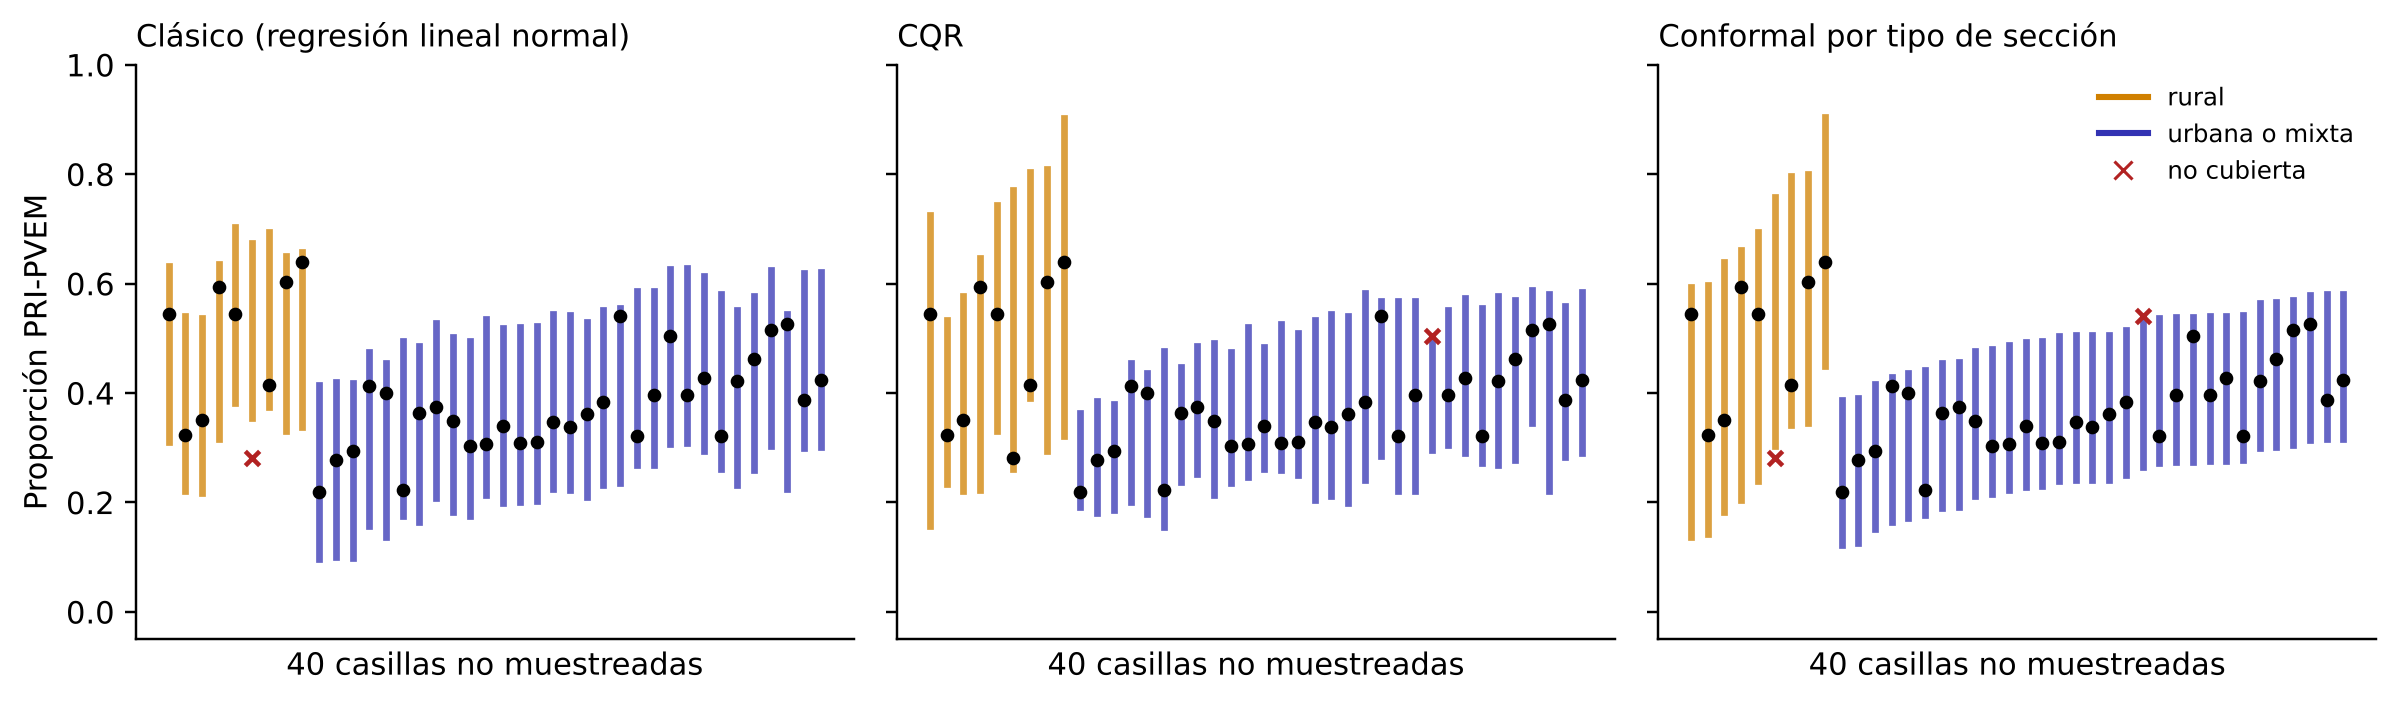
\includegraphics[width=\textwidth]{figuras/intervalos2012.png}
\end{center}
\dest{Lectura.} (i) El intervalo clásico cubre 90.3\% en total: aquí la muestra es grande y los
errores no están lejos de la normal, así que funciona marginalmente; pero su ancho es el mismo en
todas las casillas y, como el conformal de un umbral, cubre de más en las urbanas y de menos en las
rurales. Su 90\% depende del modelo; el del conformal, sólo del sorteo. (ii) Los cuantiles sin
calibrar cubren 81\%: un modelo de cuantiles, por bueno que sea, no garantiza su nivel en muestra
finita. (iii) CQR toma esos mismos cuantiles y, con un solo paso de calibración, recupera 90\% y
conserva la adaptación: ancho 0.28 en urbanas y 0.41 en rurales. (iv) Calibrar por tipo de sección es
lo único que da 90\% en cada grupo. Errores Monte Carlo de las coberturas menores a 0.4 puntos.

\subsection{Verificación con las casillas de 2012}\label{sec:beta2012}\lamina{29}
La misma población permite ver la Beta de la sección~\ref{sec:beta} con datos reales. Aquí
no se usa el diseño del conteo rápido (7,500 casillas), sino uno hecho para medir $Q$ con
exactitud. El diseño es éste:
\begin{enumerate}
\item Respuesta: proporción del voto para PRI-PVEM en la casilla. Covariables: estado, tipo de
sección, ruralidad, tamaño de la sección, tipo de casilla y lista nominal.
\item Entrenamiento: una muestra al azar de 2,000 casillas y un boosting de regresión. El modelo se
fija una vez.
\item Puntaje: $|y-\fhat(x)|$, calculado para las 141,100 casillas restantes. Esa población hace de
distribución: un caso nuevo es una casilla al azar de ella.
\item Para $n\in\{19,99,999\}$ se repite 3,000 veces: sacar al azar $n$ casillas para calibrar,
calcular $\qhat=S_{(k)}$ y medir $Q$ como la fracción \emph{exacta} de las casillas restantes cuyo
puntaje queda por debajo de $\qhat$.
\end{enumerate}
Como cada calibración es una muestra al azar de una población grande, los puntajes son prácticamente
i.i.d.\ (Proposición~\ref{prop:urna}); sólo 0.3\% de los puntajes se repiten. Los resultados:
\begin{center}
\begin{tabular}{rcccccc}
\toprule
$n$ & Media de $Q$ & Teórica & DE de $Q$ & Teórica & $\Prob(Q<0.85)$ & Teórica\\
\midrule
19 & 0.897 & 0.900 & 0.0658 & 0.0655 & 0.209 & 0.198\\
99 & 0.901 & 0.900 & 0.0295 & 0.0299 & 0.055 & 0.060\\
999 & 0.900 & 0.900 & 0.0095 & 0.0095 & 0.000 & $<0.001$\\
\bottomrule
\end{tabular}
\end{center}
\begin{center}
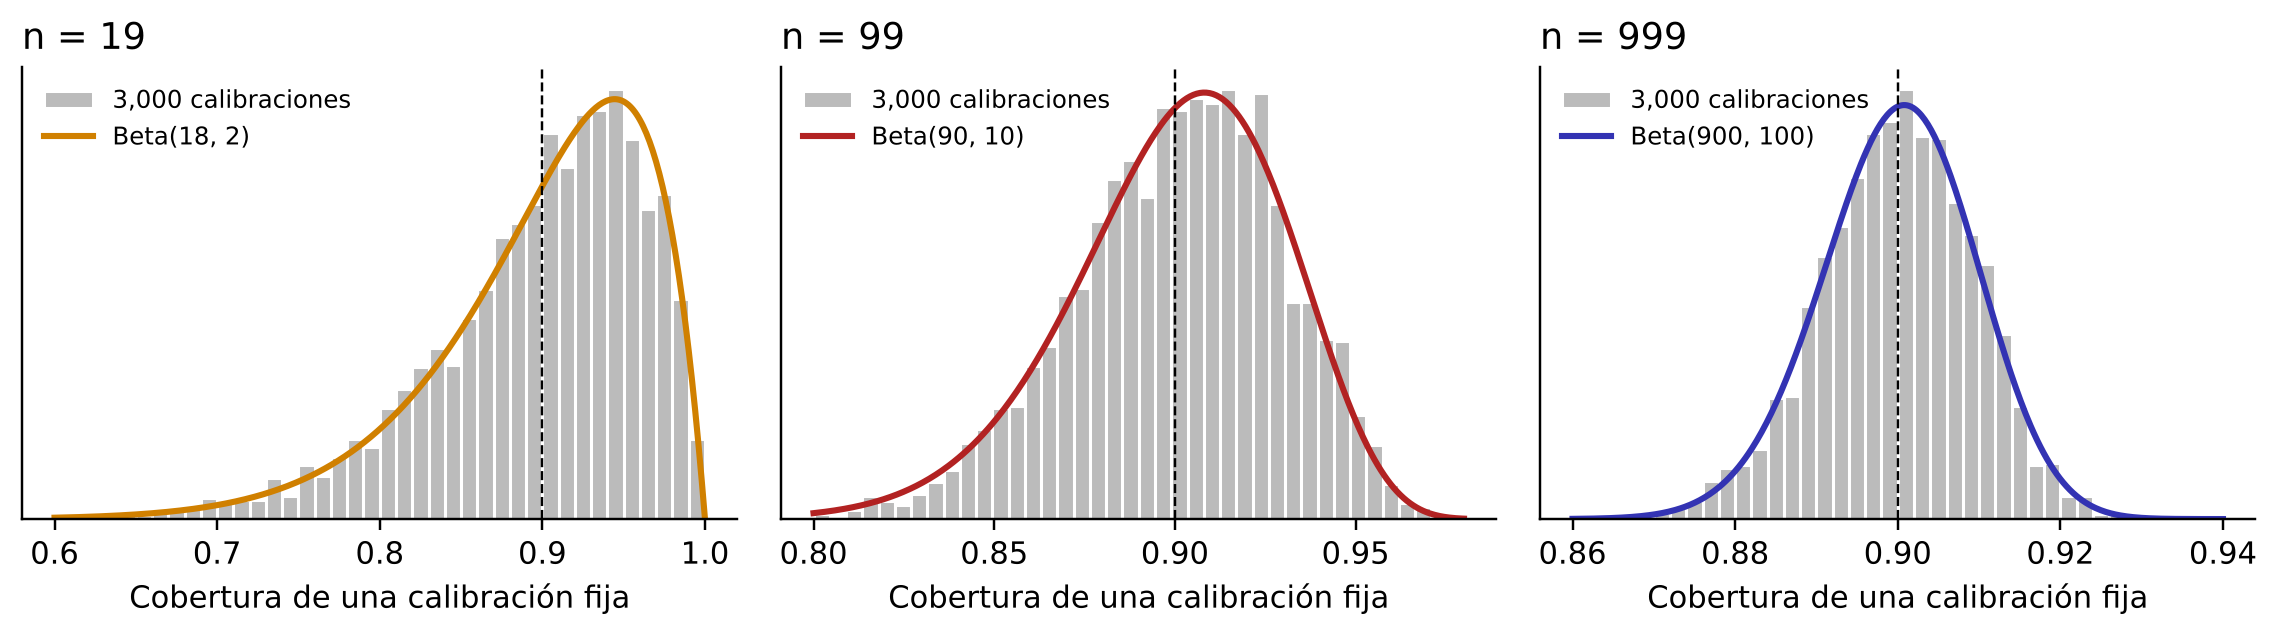
\includegraphics[width=\textwidth]{figuras/beta_2012.png}
\end{center}
Las diferencias son del tamaño del error Monte Carlo (con 3,000 réplicas, el de la media es cercano a
$0.066/\sqrt{3000}\approx0.0012$ para $n=19$). El mensaje: en 2012 la intercambiabilidad la produce
el muestreo al azar, y la teoría se cumple en datos electorales reales. En 2018 la calibración no es
una muestra al azar, sino lo que llegó primero (sección~\ref{sec:ine}).


% =====================================================================
\section{Complemento: cuando el sorteo no basta, el conteo de 2018}\label{sec:ine}
En la noche de la elección
la muestra no llega completa, y las casillas que llegan primero no son una muestra al azar de las que
faltan.

\subsection{El problema}
En 2018 el INE sorteó una muestra estratificada de 7,787 casillas en 350 estratos. Los resultados
llegan por remesas durante la noche y el comité publica antes de tener toda la muestra; la estimación
de las 22:30 usó 5,254 casillas. La pregunta conforme es local: ¿qué proporción de votos tendrá AMLO
en una casilla que todavía no llega? No es un intervalo para el porcentaje nacional.

\dest{El cambio de escenario.} Dentro de cada estrato las casillas se sortean sin reemplazo: es la
urna de la Proposición~\ref{prop:urna}. Pero la calibración no es una muestra al azar: son las
casillas que llegaron primero. Si la llegada depende del tipo de casilla, el caso nuevo (una
pendiente) no es intercambiable con la calibración. Repartir al azar las recibidas entre entrenamiento
y calibración no lo arregla: la asimetría está entre recibidas y pendientes.

\subsection{Datos}
Paquete \texttt{quickcountmx} del comité técnico. Se usan las 7,754 casillas de la muestra con hora de
llegada registrada: 6,286 enviaron su remesa durante la noche y 1,468 nunca llegaron pero tienen
cómputo distrital. La respuesta es la proporción para AMLO, con numerador y denominador siempre de la
misma fuente (remesa o cómputo); remesa y cómputo coinciden en la mayoría de las casillas pero no en
todas. Las covariables son censales y de diseño (tipo de sección, tipo de casilla, entidad, lista
nominal y proporciones de vivienda con internet, piso de tierra, lavadora, refrigerador y celular),
sin votos.

\dest{Procedimiento.} En cada corte (20:00, 21:00, 22:00), las remesas recibidas se reparten al azar
mitad para entrenar un boosting de regresión y mitad para calibrar; puntaje $|y-\fhat(x)|$,
$\alpha=0.10$; 20 repeticiones del reparto.

\subsection{Resultados}
\begin{center}
\begin{tabular}{lccc}
\toprule
Casillas evaluadas & 20:00 & 21:00 & 22:00\\
\midrule
Calibración (mitad de las recibidas) & 419 & 1,371 & 2,269\\
\midrule
Tardías, evaluadas con su remesa & 88.5\% & 88.2\% & 89.2\%\\
Tardías, evaluadas con su cómputo & 88.9\% & 88.4\% & 89.8\%\\
Nunca llegaron (cómputo) & 82.1\% & 81.6\% & 82.3\%\\
Todas las pendientes (cómputo) & 87.5\% & 86.4\% & 86.3\%\\
\quad rurales & 75.8\% & 72.2\% & 71.2\%\\
\quad urbanas & 91.2\% & 91.4\% & 92.6\%\\
\bottomrule
\end{tabular}
\end{center}
Errores Monte Carlo de 0.2 a 0.5 puntos. La fila ``nunca llegaron'' se obtiene por diferencia: las
pendientes con cómputo son las tardías más las 1,468 que nunca llegaron.

\dest{Lectura.} Cambiar remesa por cómputo en las mismas casillas casi no mueve la cobertura: la
medición no es el problema. La caída hasta 86\% viene sobre todo de las casillas que nunca llegaron,
que se cubren alrededor de 82\%: son las que menos se parecen a la calibración.

\subsection{Un control con p-valores: ¿qué parte es la llegada?}
La brecha rural (71--76\%) es tentadora de atribuir a la llegada. El control de la
sección~\ref{sec:pvalores} muestra que no: si las mismas 6,286 reportantes se reparten \emph{al azar},
ignorando la hora, las rurales se siguen cubriendo alrededor de 76\%. La brecha rural es el fenómeno
de ``marginal no es por grupo'', como en imágenes y crédito. Lo que sí produce la llegada es que la
cobertura \emph{global} baje de 90\% a 88\% entre las reportantes tardías, y a 86\% al incluir las
que nunca llegaron.

\subsection{Extensiones que se mencionan}
\dest{Calibración por grupo.} Un umbral para rurales y otro para urbanas, como en la
sección~\ref{sec:mondrian}. Arreglaría la cobertura por tipo de sección si dentro de cada tipo la
llegada no seleccionara; no corrige por sí sola la llegada.

\dest{Conformal ponderado (Tibshirani, Barber, Candès y Ramdas, 2019).} Si calibración y caso nuevo
difieren \emph{sólo} en la distribución de $X$ (la calibración es i.i.d.\ con marginal $P_X$, el caso
nuevo es independiente con marginal $\widetilde P_X\ll P_X$, ambos con la misma ley de $Y\mid X$, y el
entrenamiento está separado), se pondera cada punto de calibración con
$w(x)=d\widetilde P_X/dP_X(x)$, incluido el peso del caso nuevo:
\[
 \mu_x=\sum_{i=1}^n\frac{w(X_i)}{W+w(x)}\delta_{S_i}+\frac{w(x)}{W+w(x)}\delta_{+\infty},\qquad
 W=\sum_{i=1}^n w(X_i),
\]
y $\qhat_w(x)$ es el cuantil $1-\alpha$ de $\mu_x$. Con pesos conocidos la cobertura vuelve a ser al
menos $1-\alpha$. Es la Proposición~\ref{prop:cuantil} con pesos: el átomo en $+\infty$ representa
al caso nuevo. Si $w(x)/(W+w(x))>\alpha$ el umbral es infinito: un caso nuevo muy distinto de la
calibración no se puede cubrir de manera informativa. En la práctica $w$ se estima y la garantía se
degrada según el error de estimación (Lei y Candès, 2021).

\dest{Cota sin intercambiabilidad (Barber, Candès, Ramdas y Tibshirani, 2023).} Con pesos fijos, la
pérdida de cobertura está acotada por cuánto cambia la distribución de los datos al intercambiar cada
punto de calibración con el nuevo, medido en variación total. Si los datos son intercambiables, la
pérdida es cero.

\dest{Sensibilidad.} Si la llegada depende del propio voto aun después de observar $X$, ningún peso
basado en $X$ lo corrige. Lo honesto sería suponer que la razón de momios de llegada verdadera
difiere de la estimada a lo más por un factor $\Gamma$ y construir conjuntos válidos para todo ese
rango (Jin, Ren y Candès, 2023). Queda como idea a futuro.

\dest{El total nacional.} No basta sumar intervalos por casilla para obtener uno nacional: faltan
cobertura conjunta, pesos y diseño. Para el total, la herramienta natural son estimadores de
diferencia o inferencia asistida por predicciones, con la misma advertencia sobre la llegada.

% =====================================================================
\section{P-valores conformes}\label{sec:pvalores}\lamina{30}
\subsection{El mismo rango, leído como prueba}
Para un caso $x$ y una respuesta candidata $y$, el \emph{p-valor conforme} es
\[
 p(x,y)=\frac{1+\#\{i\le n:\ S_i\ge s_T(x,y)\}}{n+1}.
\]
Es la proporción de puntajes, contando al candidato, que son al menos tan raros como el suyo. Contrasta
la hipótesis ``$(x,y)$ es intercambiable con la calibración''. No es un tema nuevo: es el rango de la
sección~\ref{sec:orden} contado desde arriba.

\begin{teorema}[validez]\label{teo:pvalor}
Si los puntajes son intercambiables dado $T$, para todo $\alpha\in(0,1)$
\[
 \Prob\{p(X_{n+1},Y_{n+1})\le\alpha\mid T\}\le\alpha .
\]
Sin empates, $p(X_{n+1},Y_{n+1})$ es uniforme en $\{1/(n+1),2/(n+1),\dots,1\}$.
\end{teorema}
\begin{proof}[Demostración sin empates]
En la respuesta verdadera, $\#\{i\le n: S_i\ge S_{n+1}\}=n-\#\{i\le n:S_i<S_{n+1}\}=n-(R_{n+1}-1)$, así
que
\[
 p(X_{n+1},Y_{n+1})=\frac{n+2-R_{n+1}}{n+1}.
\]
Como $R_{n+1}$ es uniforme en $\{1,\dots,n+1\}$ (Lema~\ref{lem:rango}), $n+2-R_{n+1}$ también lo es, y
el p-valor es uniforme en la rejilla $\{j/(n+1)\}_{j=1}^{n+1}$. Exactamente $\lfloor\alpha(n+1)\rfloor$
puntos de la rejilla son $\le\alpha$, así que
$\Prob(p\le\alpha\mid T)=\lfloor\alpha(n+1)\rfloor/(n+1)\le\alpha$.
\end{proof}
\begin{proof}[Demostración con empates]
Con el desempate lexicográfico de la sección~\ref{sec:teorema}, sea
$p^*=\bigl(1+\#\{i\le n:(S_i,U_i)>(S_{n+1},U_{n+1})\}\bigr)/(n+1)$, que es uniforme en la rejilla por
el caso sin empates. Si $(S_i,U_i)>(S_{n+1},U_{n+1})$ entonces $S_i\ge S_{n+1}$; así $p\ge p^*$ y
$\Prob(p\le\alpha)\le\Prob(p^*\le\alpha)\le\alpha$.
\end{proof}

\begin{proposicion}[el conjunto es la inversión de la prueba]
Para todo $x$, $\ C(x)=\{y:\ p(x,y)>\alpha\}$.
\end{proposicion}
\begin{proof}
Sea $s=s_T(x,y)$ y $m=\lfloor\alpha(n+1)\rfloor$. Como los conteos son enteros,
\[
 p(x,y)>\alpha\iff\#\{i:S_i\ge s\}>\alpha(n+1)-1\iff\#\{i:S_i\ge s\}\ge m
 \iff\#\{i:S_i<s\}\le n-m .
\]
Por otro lado $k=\lceil(n+1)(1-\alpha)\rceil=n+1-\lfloor\alpha(n+1)\rfloor=n+1-m$, porque
$\lceil N-a\rceil=N-\lfloor a\rfloor$ para $N$ entero. Así la condición es $\#\{i:S_i<s\}\le k-1$. Si
$k\le n$, por el Lema~\ref{lem:conteo} equivale a $s\le S_{(k)}=\qhat$. Si $k=n+1$, la condición
siempre se cumple, como $s\le\qhat=+\infty$.
\end{proof}
El conjunto que se usó en toda la charla es, entonces, el conjunto de respuestas que una prueba de
nivel $\alpha$ no rechaza: la misma dualidad entre pruebas e intervalos de confianza de la
estadística clásica.

\subsection{Para revisar el supuesto}
Cuando la respuesta ya se observó, el p-valor de un caso dice qué tan raro es frente a la
calibración. Si la intercambiabilidad se cumple, cada p-valor cumple el Teorema~\ref{teo:pvalor},
así que en un conjunto grande de casos nuevos la proporción con $p\le\alpha$ debe quedar cerca de
$\alpha$ (o debajo), para todo $\alpha$. Una curva de esa proporción contra $\alpha$ que se despega
de la diagonal es evidencia contra el supuesto. Los p-valores de casos que comparten calibración no
son independientes, así que es un diagnóstico, no una prueba formal; las pruebas formales de
intercambiabilidad en línea usan martingalas conformes (Vovk, Gammerman y Shafer, 2005).

\dest{Complemento: el conteo rápido de 2012.} Con el diseño de la sección~\ref{sec:conteo2012}, se calculan
los p-valores de las casillas no muestreadas, con la calibración completa (un solo umbral) o con la
calibración de su tipo de sección (un umbral por grupo).
\begin{center}
\begin{tabular}{lccc}
\toprule
Proporción con $p\le0.10$ & Todas & Rurales & Urbanas\\
\midrule
Un solo umbral & 10.0\% & 24.4\% & 5.2\%\\
Un umbral por grupo & 10.0\% & 10.0\% & 10.0\%\\
\bottomrule
\end{tabular}
\end{center}
\begin{center}
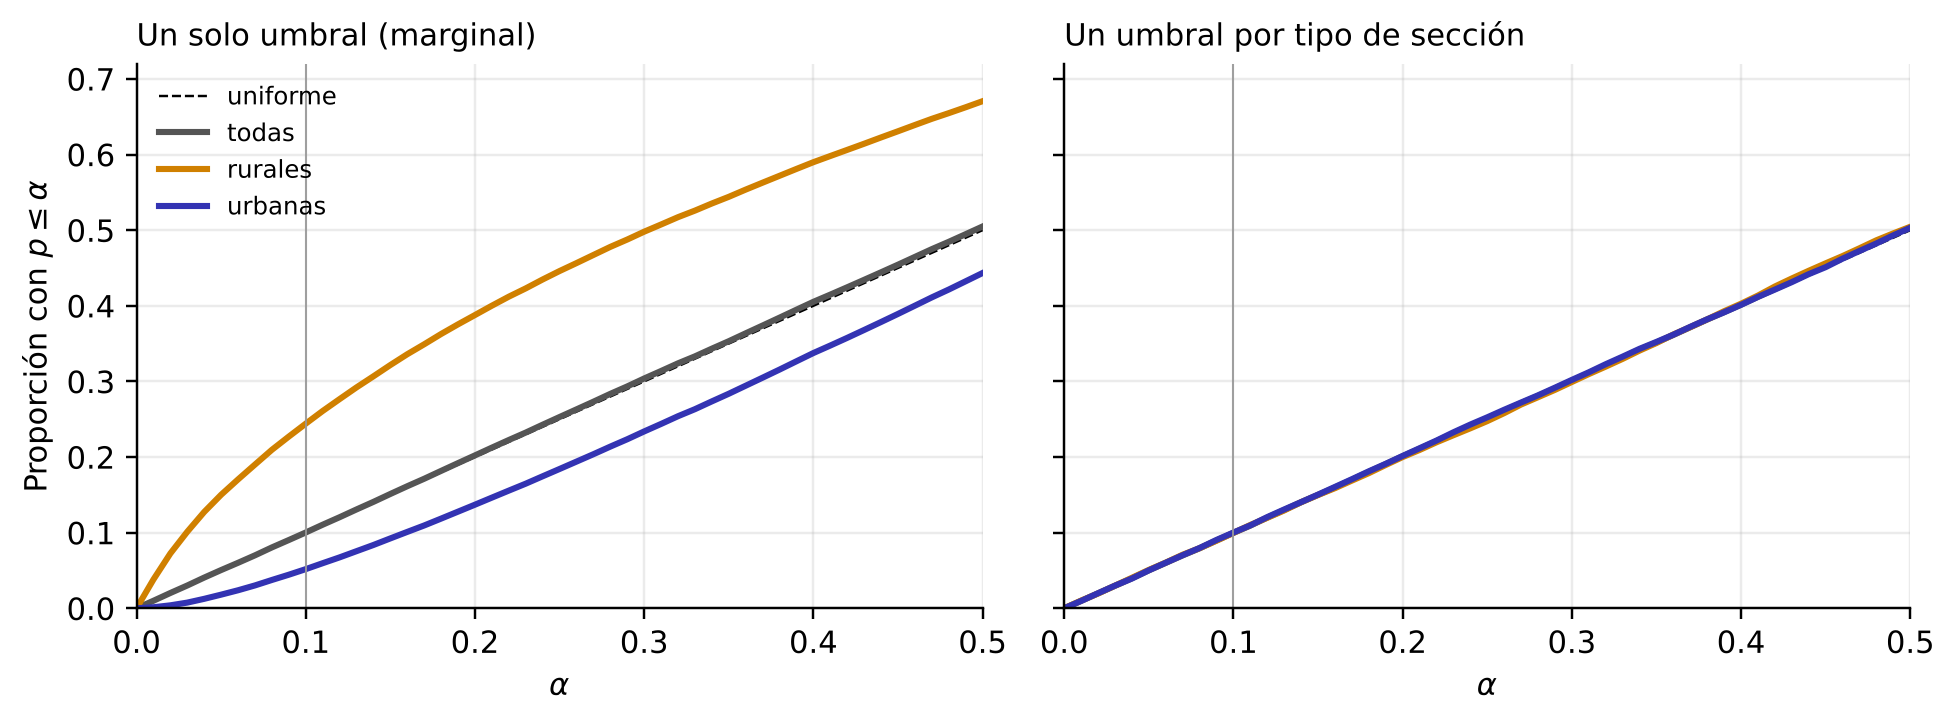
\includegraphics[width=0.95\textwidth]{figuras/conteo2012_pvalores.png}
\end{center}
Con un solo umbral, la curva global cae en la diagonal, como predice el teorema, pero las rurales
quedan muy por encima: la intercambiabilidad vale para la población completa, no dentro de cada
grupo con una calibración común. Con un umbral por grupo, las tres curvas caen en la diagonal. Con
esto se cierra el círculo: el rango que construyó el conjunto es el mismo que permite revisar el
supuesto.

\dest{En 2018, con la llegada real.} Corte de 21:00, reportantes tardías, respuesta y calibración en remesa.
Se comparan dos esquemas con los mismos tamaños (1,371 de calibración, 3,545 de prueba):
\emph{llegada real}, y un \emph{control} en que las 6,286 reportantes se reparten al azar ignorando la
hora. Veinte repeticiones.
\begin{center}
\begin{tabular}{lccc}
\toprule
Proporción con $p\le0.10$ & Todas & Rurales & Urbanas\\
\midrule
Control al azar & 9.7\% & 24.2\% & 5.9\%\\
Llegada real & 11.8\% & 25.7\% & 8.4\%\\
\bottomrule
\end{tabular}
\end{center}
\begin{center}
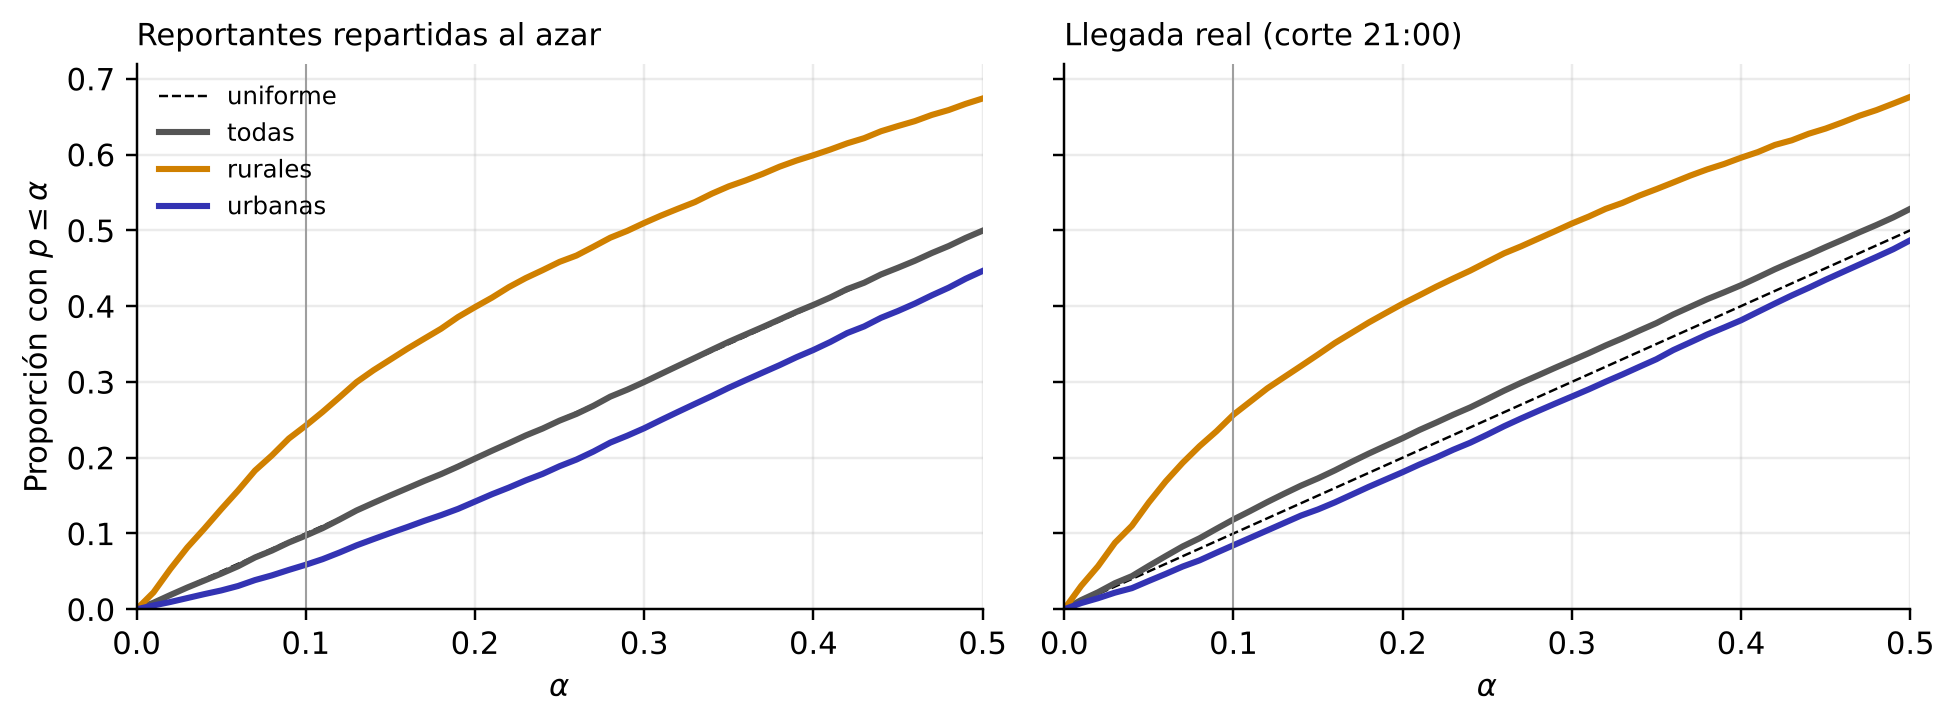
\includegraphics[width=0.95\textwidth]{figuras/ine_pvalores.png}
\end{center}
Con el control, la curva global cae en la diagonal, como predice el teorema. Con la llegada real se
despega: 11.8\% de p-valores menores que 0.10. Las rurales quedan muy por encima \emph{en los dos
esquemas}: su mala cobertura no la causa la llegada, sino que la garantía es marginal, igual que en
2012.

\dest{Conformal completo.} Split sacrifica datos: unos sólo entrenan y otros sólo calibran. La versión
original no parte los datos: para cada candidata $y$ se ajusta el modelo con los $n+1$ puntos
$(X_1,Y_1),\dots,(X_n,Y_n),(x,y)$, se calculan los $n+1$ puntajes y se incluye $y$ si su p-valor
supera $\alpha$. Tiene la misma garantía si el ajuste trata simétricamente a los $n+1$ puntos; el
costo es reajustar para cada candidata. Jackknife+ es una alternativa intermedia, con garantía
general $1-2\alpha$ (Barber et al., 2021).

% =====================================================================
\section{Preguntas probables}
\begin{description}[style=nextline,leftmargin=1em,font=\normalfont\bfseries]
\item[¿Cada conjunto tiene 90\% de probabilidad de cubrir?]
No. La garantía promedia sobre calibración y caso nuevo. Para una calibración fija la cobertura es un
número que, bajo puntajes i.i.d.\ continuos, varía con ley Beta (sección~\ref{sec:beta}); en 2012 se
ve con datos reales.
\item[¿Qué pasa si el modelo está mal?]
La garantía marginal se conserva mientras haya intercambiabilidad. Empeora la utilidad (conjuntos más
grandes) y puede haber grupos mal cubiertos.
\item[¿Funciona con cualquier modelo?]
Sí: redes, boosting, modelos de lenguaje. Sólo se necesita un puntaje fijado antes de calibrar.
\item[¿Cómo elijo el puntaje?]
La garantía no depende de él; el tamaño sí. Se elige por utilidad, con datos de entrenamiento o
validación, nunca con la calibración (sección~\ref{sec:puntajes}).
\item[¿La logística no tiene ya sus probabilidades?]
Sí, estimadas. El conjunto oráculo tiene garantía para cada $x$ sólo con la probabilidad verdadera; el
plug-in no la hereda.
\item[¿Por qué no bootstrap?]
Sus justificaciones suelen ser asintóticas y dependen de regularidad. Conformal es exacto para $n$
finita bajo intercambiabilidad.
\item[¿Cuántos datos de calibración necesito?]
Al menos $1/\alpha-1$ para un umbral finito. Para que una corrida no se aleje del nominal, cientos:
con $n=999$ la desviación estándar de la cobertura es 0.0095.
\item[¿Puedo escoger el mejor modelo mirando la calibración?]
No, sin perder el teorema. La selección debe hacerse con entrenamiento o validación aparte.
\item[¿Se puede tener cobertura para cada $x$?]
No sin supuestos (teorema de imposibilidad). Sí por grupos definidos de antemano, calibrando en cada
uno (sección~\ref{sec:mondrian}).
\item[¿Y con empates?]
La cota inferior se conserva; la superior puede fallar. Ocurre con modelos de árboles.
\item[¿Y con series de tiempo?]
La intercambiabilidad falla. Hay variantes en línea que ajustan $\alpha$ sobre la marcha y garantizan
cobertura promedio de largo plazo (Gibbs y Candès, 2021).
\item[¿Cómo sé si mis datos son intercambiables?]
Por cómo se obtuvieron: un sorteo, una partición al azar. Los p-valores conformes sirven para detectar
violaciones, no para certificarla (sección~\ref{sec:pvalores}).
\item[¿El caso del INE demuestra que la llegada causó la caída?]
Muestra que la cobertura global baja con la llegada real y no con el control al azar, y que la caída
mayor está en las casillas que nunca llegaron. La brecha rural, en cambio, aparece también al azar.
\item[¿Es frecuentista o bayesiano?]
La garantía es frecuentista. Una predictiva bayesiana puede usarse como puntaje: si el modelo es
correcto da intervalos parecidos a los bayesianos, y si no, conserva la cobertura (Fong y Holmes,
2021).
\end{description}

\clearpage
\appendix
\section{Cuántos datos se usaron en cada ejemplo}\label{sec:datos}
En todos los ejemplos $\alpha=0.10$ y el cuantil es $S_{(k)}$ con $k=\lceil(n+1)(1-\alpha)\rceil$.
``Réplicas'' es el número de particiones o sorteos al azar; las cifras reportadas son sus medias.
\begin{center}
\footnotesize\renewcommand{\arraystretch}{1.25}\setlength{\tabcolsep}{3pt}
\begin{tabular}{>{\raggedright}p{2.0cm}>{\raggedright}p{2.0cm}>{\raggedright}p{1.5cm}>{\raggedright}p{2.4cm}>{\raggedright}p{1.9cm}>{\raggedright}p{1.2cm}>{\raggedright\arraybackslash}p{2.8cm}}
\toprule
Ejemplo & Total & Entrena & Calibra & Evalúa & Réplicas & Modelo y puntaje\\
\midrule
Dígitos & 1,797 imágenes de $8\times8$, tres niveles de ruido al azar & 600 & 500 (\(k=451\)) & 697 & 100 & Logística multinomial; $1-\phat_y(x)$\\
Crédito & 30,000 clientes, 22.1\% incumplen & 18,000 (60\%) & 6,000 (20\%): $\approx$4,670 pagan y $\approx$1,330 incumplen; por clase, un $\qhat$ con cada grupo & 6,000 (20\%) & 20 & Logística sin penalizar y boosting (HistGB); $1-\phat_y(x)$\\
Elecciones 2012, conteo & 143,100 casillas; se sortean 7,500 & 3,750 & 3,750 (\(k=3{,}376\)): $\approx$2,491 urbanas, 422 mixtas, 804 rurales; 33 sin tipo & 135,600 no muestreadas & 20 & Boosting de regresión; $|y-\fhat(x)|$\\
Intervalos 2012 & los mismos 7,500 sorteados & 3,750 (el lineal usa las 7,500) & 3,750 (CQR y conformal) & 135,600 & 20 & Lineal normal, cuantiles 5\%/95\%, CQR, conformal\\
Beta 2012 & 143,100 casillas & 2,000 (una vez) & $n=19$, 99 y 999 al azar de las 141,100 restantes & las $141{,}100-n$ restantes (exacto) & 3,000 por cada $n$ & Boosting de regresión; $|y-\fhat(x)|$\\
P-valores 2018 & 7,754 casillas de la muestra con hora de llegada & mitad de las recibidas & 1,371 (corte de 21:00) & 3,545 pendientes & 20 & Boosting de regresión; $|y-\fhat(x)|$\\
INE 2018, complemento & 7,754 casillas & mitad de las recibidas & 419, 1,371 y 2,269 (cortes de 20, 21 y 22~h) & pendientes & 20 & Boosting de regresión; $|y-\fhat(x)|$\\
\bottomrule
\end{tabular}
\end{center}
Los valores de $k$: con $n=500$, $k=\lceil501\times0.9\rceil=451$; con $n=3{,}750$,
$k=\lceil3{,}751\times0.9\rceil=3{,}376$; con $n=19$, 99 y 999, $k=18$, 90 y 900. En la calibración
por grupo de 2012 cada grupo usa su propio $n$: urbanas $k\approx2{,}243$, mixtas $k\approx381$,
rurales $k\approx725$. En crédito por clase, $k\approx4{,}207$ para los que pagan y $k\approx1{,}196$
para los que incumplen.

\clearpage
\section{Datos y programas}
Todas las rutas son relativas a la carpeta \path{aplicaciones} del repositorio.
\begin{center}
\small
\begin{tabular}{p{4.2cm}p{5.2cm}p{5.6cm}}
\toprule
Resultado & Programa & Datos\\
\midrule
Imágenes (sección~\ref{sec:imagenes}) & \path{01_digitos/imagenes.py} & dígitos de \texttt{scikit-learn}\\
Beta con 2012 (sección~\ref{sec:beta2012}) & \path{03_conteo_2012/beta2012.py} & \texttt{quickcountmx}, \texttt{nal\_2012}\\
Conteo 2012 (sección~\ref{sec:conteo2012}) & \path{03_conteo_2012/conteo2012.py} & ídem\\
Comparación de intervalos 2012 & \path{03_conteo_2012/intervalos2012.py} & ídem\\
Crédito marginal & \path{02_credito/credito.py} & UCI (ver \path{02_credito/README.md})\\
Crédito por clase & \path{02_credito/credito_mondrian.py} & ídem\\
INE, coberturas & \path{04_ine_2018/ine.py} & \texttt{quickcountmx} (commit 86c75437)\\
INE, p-valores & \path{04_ine_2018/ine_pvalores.py} & ídem\\
\bottomrule
\end{tabular}
\end{center}
Los resultados están en la carpeta \path{resultados/} de cada aplicación. Las cifras de crédito e INE se reprodujeron
exactamente al reejecutar los programas con los datos originales.

\section*{Fuentes}
\addcontentsline{toc}{section}{Fuentes}
\small
\textbf{Para estudiar, en este orden}
\begin{enumerate}
\item Angelopoulos, A. N. y Bates, S. (2023). Conformal prediction: A gentle introduction.
\emph{Foundations and Trends in Machine Learning}, 16(4), 494--591.
\item Lei, J., G'Sell, M., Rinaldo, A., Tibshirani, R. J. y Wasserman, L. (2018). Distribution-free
predictive inference for regression. \emph{JASA}, 113, 1094--1111.
\item Angelopoulos, A. N., Barber, R. F. y Bates, S. \emph{Theoretical Foundations of Conformal
Prediction}. Cambridge University Press (arXiv:2411.11824).
\item Tibshirani, R. J., Barber, R. F., Candès, E. J. y Ramdas, A. (2019). Conformal prediction under
covariate shift. \emph{NeurIPS}.
\end{enumerate}
\textbf{Fundamentos}
\begin{itemize}
\item Vovk, V., Gammerman, A. y Shafer, G. (2005; 2a ed. 2022). \emph{Algorithmic Learning in a Random
World}. Springer.
\item Shafer, G. y Vovk, V. (2008). A tutorial on conformal prediction. \emph{JMLR}, 9, 371--421.
\item Vovk, V. (2012). Conditional validity of inductive conformal predictors. \emph{ACML}, PMLR 25.
\end{itemize}
\textbf{Puntajes}
\begin{itemize}
\item Romano, Y., Patterson, E. y Candès, E. J. (2019). Conformalized quantile regression.
\emph{NeurIPS}.
\item Sadinle, M., Lei, J. y Wasserman, L. (2019). Least ambiguous set-valued classifiers with bounded
error levels. \emph{JASA}, 114, 223--234.
\item Romano, Y., Sesia, M. y Candès, E. J. (2020). Classification with valid and adaptive coverage.
\emph{NeurIPS}.
\item Chernozhukov, V., Wüthrich, K. y Zhu, Y. (2021). Distributional conformal prediction.
\emph{PNAS}, 118(48).
\item Fong, E. y Holmes, C. (2021). Conformal Bayesian computation. \emph{NeurIPS}.
\end{itemize}
\textbf{Cobertura condicional}
\begin{itemize}
\item Lei, J. y Wasserman, L. (2014). Distribution-free prediction bands for non-parametric
regression. \emph{JRSS-B}, 76(1).
\item Foygel Barber, R., Candès, E. J., Ramdas, A. y Tibshirani, R. J. (2021). The limits of
distribution-free conditional predictive inference. \emph{Information and Inference}, 10(2).
\item Gibbs, I., Cherian, J. J. y Candès, E. J. (2025). Conformal prediction with conditional
guarantees. \emph{JRSS-B}, 87(4).
\end{itemize}
\textbf{Sin intercambiabilidad}
\begin{itemize}
\item Lei, L. y Candès, E. J. (2021). Conformal inference of counterfactuals and individual treatment
effects. \emph{JRSS-B}, 83(5).
\item Barber, R. F., Candès, E. J., Ramdas, A. y Tibshirani, R. J. (2021). Predictive inference with
the jackknife+. \emph{Annals of Statistics}, 49(1), 486--507.
\item Barber, R. F., Candès, E. J., Ramdas, A. y Tibshirani, R. J. (2023). Conformal prediction beyond
exchangeability. \emph{Annals of Statistics}, 51(2), 816--845.
\item Jin, Y., Ren, Z. y Candès, E. J. (2023). Sensitivity analysis of individual treatment effects: A
robust conformal inference approach. \emph{PNAS}, 120(6).
\item Gibbs, I. y Candès, E. J. (2021). Adaptive conformal inference under distribution shift.
\emph{NeurIPS}.
\end{itemize}
\textbf{Datos}
\begin{itemize}
\item Yeh, I.-C. y Lien, C.-H. (2009). The comparisons of data mining techniques for the predictive
accuracy of probability of default of credit card clients. \emph{Expert Systems with Applications},
36(2), 2473--2480.
\item Alpaydin, E. y Kaynak, C. (1998). Optical recognition of handwritten digits. UCI Machine Learning
Repository.
\item INE (2018). Informe final del Comité Técnico Asesor de los Conteos Rápidos. Paquete
\texttt{quickcountmx} (COTECORA).
\item Anzarut, M., González, F. y Ortiz, T. (2019). A heavy-tailed multilevel mixture model for the
quick count in the Mexican elections of 2018.
\end{itemize}
\end{document}
